\documentclass[../the.tex]{subfiles}


\begin{document}
{\fontsize{13}{12} \selectfont
Trong chương này tiền hành đánh giá và thảo luận kết quả. Các mô hình sẽ được đánh giá dựa vào số lượng tham số sử dụng, tốc độ FPS và độ chính xác mAP50.
Nghiên cứu sẽ tiến hành đánh giá các mô hình dựa vào bộ dữ liệu 1, 2 đã đề cập ở phần \ref{sec:dataset} lần lượt được gọi là Thực nghiệm 1, 2, 3.
Các tập xác thực được tạo từ $20\%$ từ bộ dữ liệu, tập thử nghiệm ($5\%$) để đánh giá kết quả trên hình ảnh thực tế ở đường phố được lấy từ tập dữ liệu TACO và tự thu thập (xem Bảng \ref{tab:datasettest}).
Các mô hình được huấn luyện trên máy tính cấu hình GPU GTX 3050 với bộ nhớ 8GB.

}

\section{Thực nghiệm 1 - Đánh giá mô hình dựa vào phát hiện rác}

 {\fontsize{13}{12} \selectfont

  Thực nghiệm 1 với mục tiêu đánh giá các mô hình dựa trên việc phát hiện đối tượng có phải là rác hay không, trong tập dữ liệu có một nhãn duy nhất là rác.
  Các mô hình được so sánh trong nhiệm vụ phát hiện đối tượng, các phương pháp tăng cường dữ liệu được cài đặt cho các mô hình là như nhau được thể hiện ở Bảng \ref{tab:thamso}.
  Các tham số còn lại cài đặt theo mặc định của mô hình, như tăng cường mosiac ở YOLOv8, focal loss ở YOLOv7 mục đích đánh giá đặc trưng riêng của các mô hình.

 }
\begin{table}[h!]
    \centering
    \begin{threeparttable}
        \caption{Kết quả thực hiện Thực nghiệm 1 - đánh giá mô hình dựa vào phát hiện rác với tập xác thực}
        \begin{tabular}{lwr{2cm}wr{2cm}wr{2cm}}
            \hline
            \textbf{Mô hình}  & \textbf{Precision} & \textbf{Recall} & \textbf{mAP50} \\ \hline
            SSD   MobileNetv2 & 0,841              & 0,595           & 0,657          \\ \hline
            YOLOv7-tiny       & 0,81               & 0,699           & 0,788          \\ \hline
            YOLOv8n           & \textbf{0,873}     & \textbf{0,727}  & \textbf{0,842} \\ \hline
        \end{tabular}
        \label{tab:thucnghiem1.1}
    \end{threeparttable}
\end{table}

\begin{table}[h!]
    \centering
    \begin{threeparttable}
        \caption{Kết quả thực hiện Thực nghiệm 1 - đánh giá mô hình dựa vào phát hiện rác với tập thử nghiệm}
        \begin{tabular}{lrrr}
            \hline
            \textbf{Mô hình} & \textbf{Precision} & \textbf{Recall} & \textbf{mAP50}  \\ \hline
            SSD MobileNetv2  & 0,712              & 0,364           & 0,427                                       \\ \hline
            YOLOv7-tiny      & 0,723              & 0,515           & 0,62                               \\ \hline
            YOLOv8n          & \textbf{0,73}      & \textbf{0,606}  & \textbf{0,713}                             \\ \hline
        \end{tabular}
        \label{tab:thucnghiem1.2}
    \end{threeparttable}
\end{table}

{\fontsize{13}{12} \selectfont

Các mô hình được huấn luyện bằng phương pháp học chuyển giao dựa trên tập dữ liệu COCO, quá trình huấn luyện là 100 epoch, ngưỡng tin cậy để đánh giá là 0.3.
Kết quả đánh giá của Thực nghiệm 1 được thể hiện ở Bảng \ref{tab:thucnghiem1.1}
và Bảng \ref{tab:thucnghiem1.2} với tập dữ liệu xác thực và tập dữ liệu thực nghiệm của các mô hình.

}

\bigskip

{\fontsize{13}{12} \selectfont

    Hình \ref{fig:thucnghiem1} cho thấy YOLOv8 đạt kết quả tốt hơn so với hai mô hình còn lại. Đối với tập xác thực, mô hình SSD MobileNetv2 có khả năng nhận dạng đúng đối tượng tốt hơn so với YOLOv7-tiny, tuy nhiên Recall của mô hình lại kém so với hai mô hình họ YOLO.
    Đối với tập dữ liệu thử nghiệm, mô hình YOLOv8n vẫn vượt rội so với những mô hình còn lại, chỉ số Precision của các mô hình không có sự chênh lệch lớn (khoảng 2\%), tuy nhiên chỉ số Recall của tất cả giảm đáng kể, giảm nhiều nhất là mô hình SSD MobileNetv2 chỉ còn 36.4\%.
    Kết quả chênh lệch giữa tập dữ liệu xác thực và tập dữ liệu thực nghiệm khoảng 10 - 25\% cho thấy việc phát hiện rác ở tự nhiên khó hơn điều kiện lí tưởng bởi chịu ảnh hưởng của môi trường xung quanh đối tượng.
    Hình \ref{fig:thucnghiem1.3} bao gồm hình ảnh gán nhãn và hình ảnh kết quả của mô hình YOLOv8.

}

\begin{figure}[H]
    \centering
    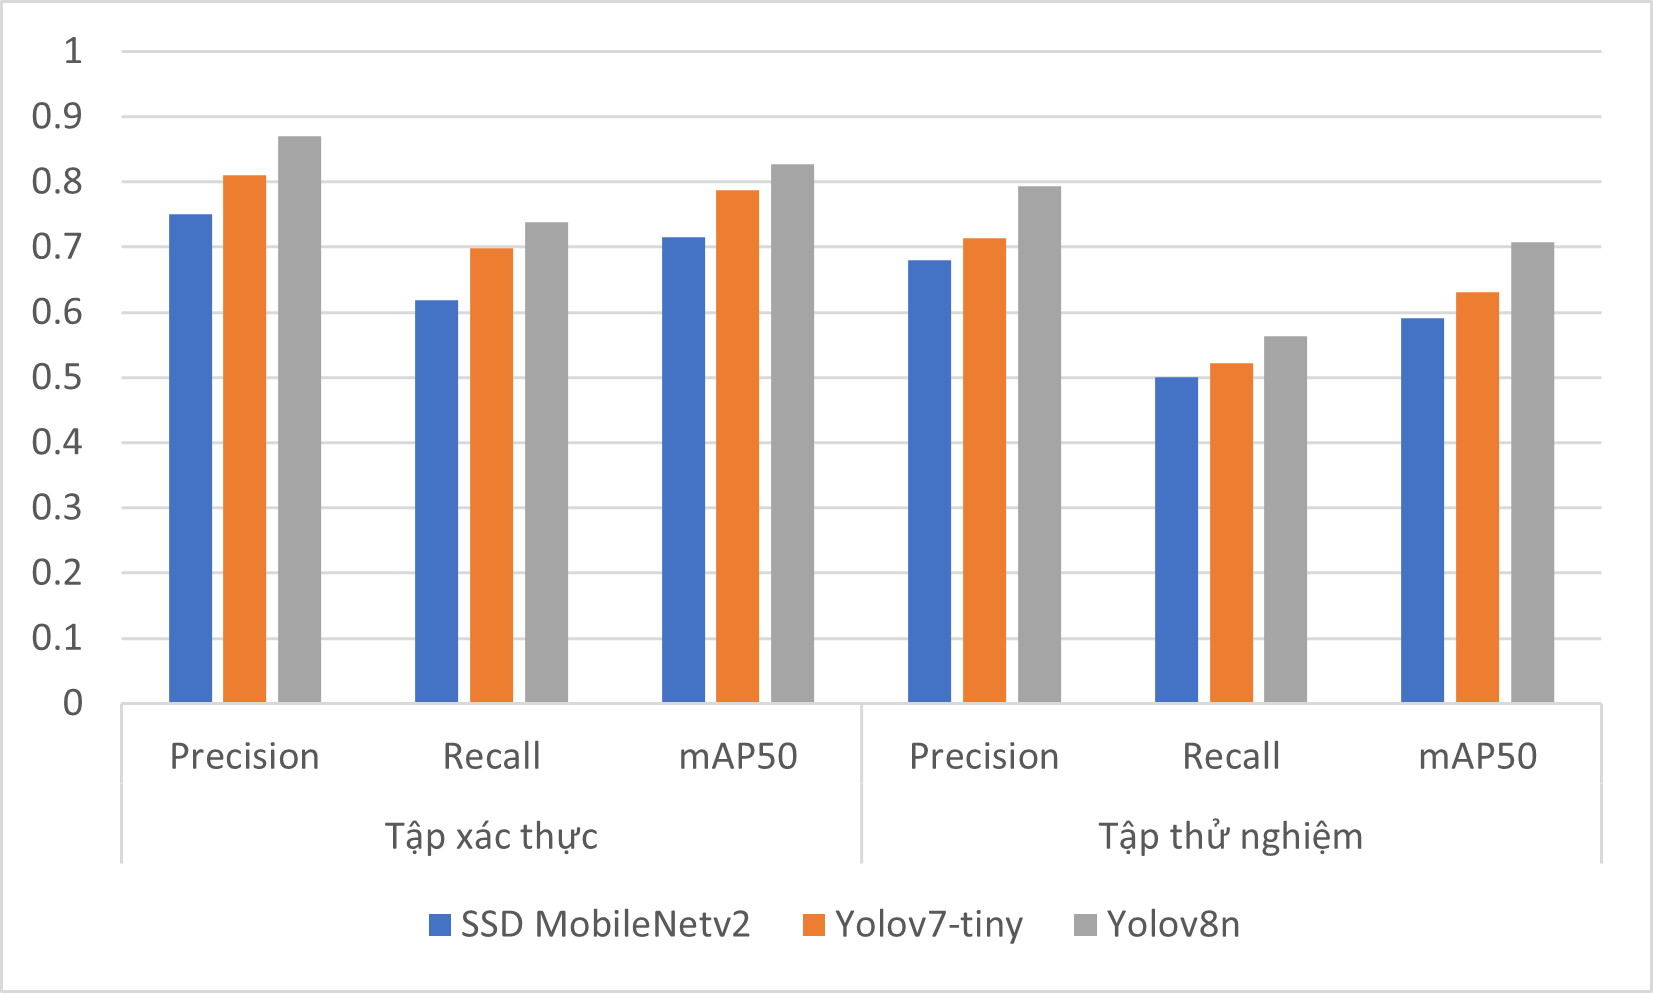
\includegraphics[width=0.7\textwidth]{thucnghiem1.png}
    \caption{Biểu đồ kết quả Thực nghiệm 1 - đánh giá mô hình dựa vào phát hiện rác}
    \label{fig:thucnghiem1}
\end{figure}


\begin{figure}[H]
    \centering
    \includegraphics[width=1.0\textwidth]{th1_data.png}
    \caption{Hình ảnh dự đoán của mô hình YOLOv8n. Bên trái là hình được gán nhãn, bên phải là hình được phát hiện bởi mô hình}
    \label{fig:thucnghiem1.3}
\end{figure}

\section{Thực nghiệm 2 - Đánh giá mô hình dựa vào phát hiện và phân loại rác}

 {\fontsize{13}{12} \selectfont

  Mô hình SSD MobileNetv2 tỏ ra không hiệu quả so với hai mô hình còn lại trong Thực nghiệm 1, vì vậy trong Thực nghiệm 2 và 3, nghiên cứu tập trung vào YOLOv7-tiny và YOLOv8n.
  Các mô hình vẫn sử dụng tham số để tăng cường dữ liệu giống như ở \ref{tab:thamso}, thực hiện trên tập dữ liệu đã đề cập ở phần \ref{sec:dataset} nhưng không bổ sung hình nền.
  Đánh giá các mô hình dựa vào chỉ số mAP50 trên từng loại rác và trung bình của tất cả, kết quả đánh giá được thể hiện Bảng \ref{tab:thucnghiem2.1} và Hình \ref{fig:thucnghiem2} ở Thực nghiệm 2.

 }

\bigskip


\begin{table}[h!]
    \centering
    \begin{threeparttable}
        \caption{Kết quả thực hiện trên tập xác thực và thử nghiệm ở Thực nghiệm 2 - đánh giá mô hình dựa vào phát hiện và phân loại rác}
        \begin{tabular}{clrwr{2cm}rrr}
            \hline
            \multicolumn{1}{l}{\textbf{Tập dữ liệu}} & \textbf{Mô hình} & \textbf{Kim loại} & \textbf{Giấy}  & \textbf{Nhựa - nilon} & \textbf{Khác}  & \textbf{Tất cả} \\ \hline
            \multirow{2}{*}{Xác thực}                & YOLOv7-tiny      & 0,689             & 0,538          & 0,538                 & 0,509          & 0,607           \\ \cline{2-7}
                                                     & YOLOv8n          & \textbf{0,759}    & \textbf{0,703} & \textbf{0,652}        & \textbf{0,581} & \textbf{0,674}  \\ \hline
            \multirow{2}{*}{Thử nghiệm}              & YOLOv7-tiny      & \textbf{0,407}    & 0,385          & 0,487                 & \textbf{0,223} & 0,376           \\ \cline{2-7}
                                                     & YOLOv8n          & 0,377             & \textbf{0,415} & \textbf{0,553}        & 0,207          & \textbf{0,388}  \\ \hline
        \end{tabular}
        \label{tab:thucnghiem2.1}
    \end{threeparttable}
\end{table}


\begin{figure}[H]
    \centering
    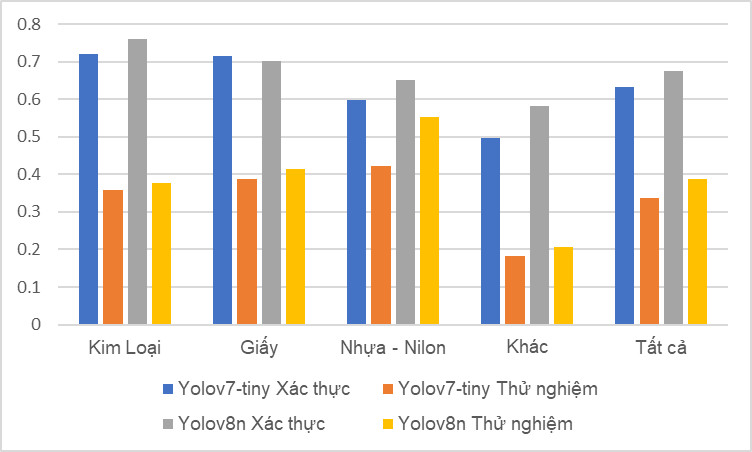
\includegraphics[width=0.8\textwidth]{thucnghiem2.1.jpg}
    \caption{Biểu đồ kết quả Thực nghiệm 2 - đánh giá mô hình dựa vào phát hiện và phân loại rác}
    \label{fig:thucnghiem2}
\end{figure}

{\fontsize{13}{12} \selectfont

Các mô hình nhận dạng tốt ở lớp "Kim loại" và thấp nhất ở lớp "Khác",
điều này có thể giải thích bằng tính đặc trưng của lớp khác quá nhiều, đa dạng về hình thể, đa phần là các rác nhỏ và khó xác định.
Ở Thực nghiệm 2, mô hình YOLOv8n có kết quả vượt trội hơn khi kiểm tra trên tập xác thực, tuy nhiên với tập dữ liệu thử nghiệm thì mô hình YOLOv7 có kết quả tốt hơn với lớp kim loại và lớp khác, nhưng tổng thể mô hình YOLOv8n vẫn tốt hơn $1,2\%$ .
Hình \ref{fig:thucnghiem2.1} cho thấy việc các hình nền dễ bị nhận dạng trở thành các đối tượng rác, trong đó có thể gồm các đối tượng như đá, các biển báo, vũng nước hoặc nhận dạng trùng lặp các hộp giới hạn gần vị trí của nhau.
Các đối tượng từ "Giấy" cũng dễ bị nhận nhầm với với rác "Khác", lớp "Kim loại" có sự ổn định cao và ít nhầm lẫn với lớp còn lại. Lớp "Giấy" và "Nhựa - nilon" dễ bị bỏ qua không thể nhận dạng vì các đối tượng bị chồng chéo lên nhau.

}


\begin{figure}[H]
    \centering
    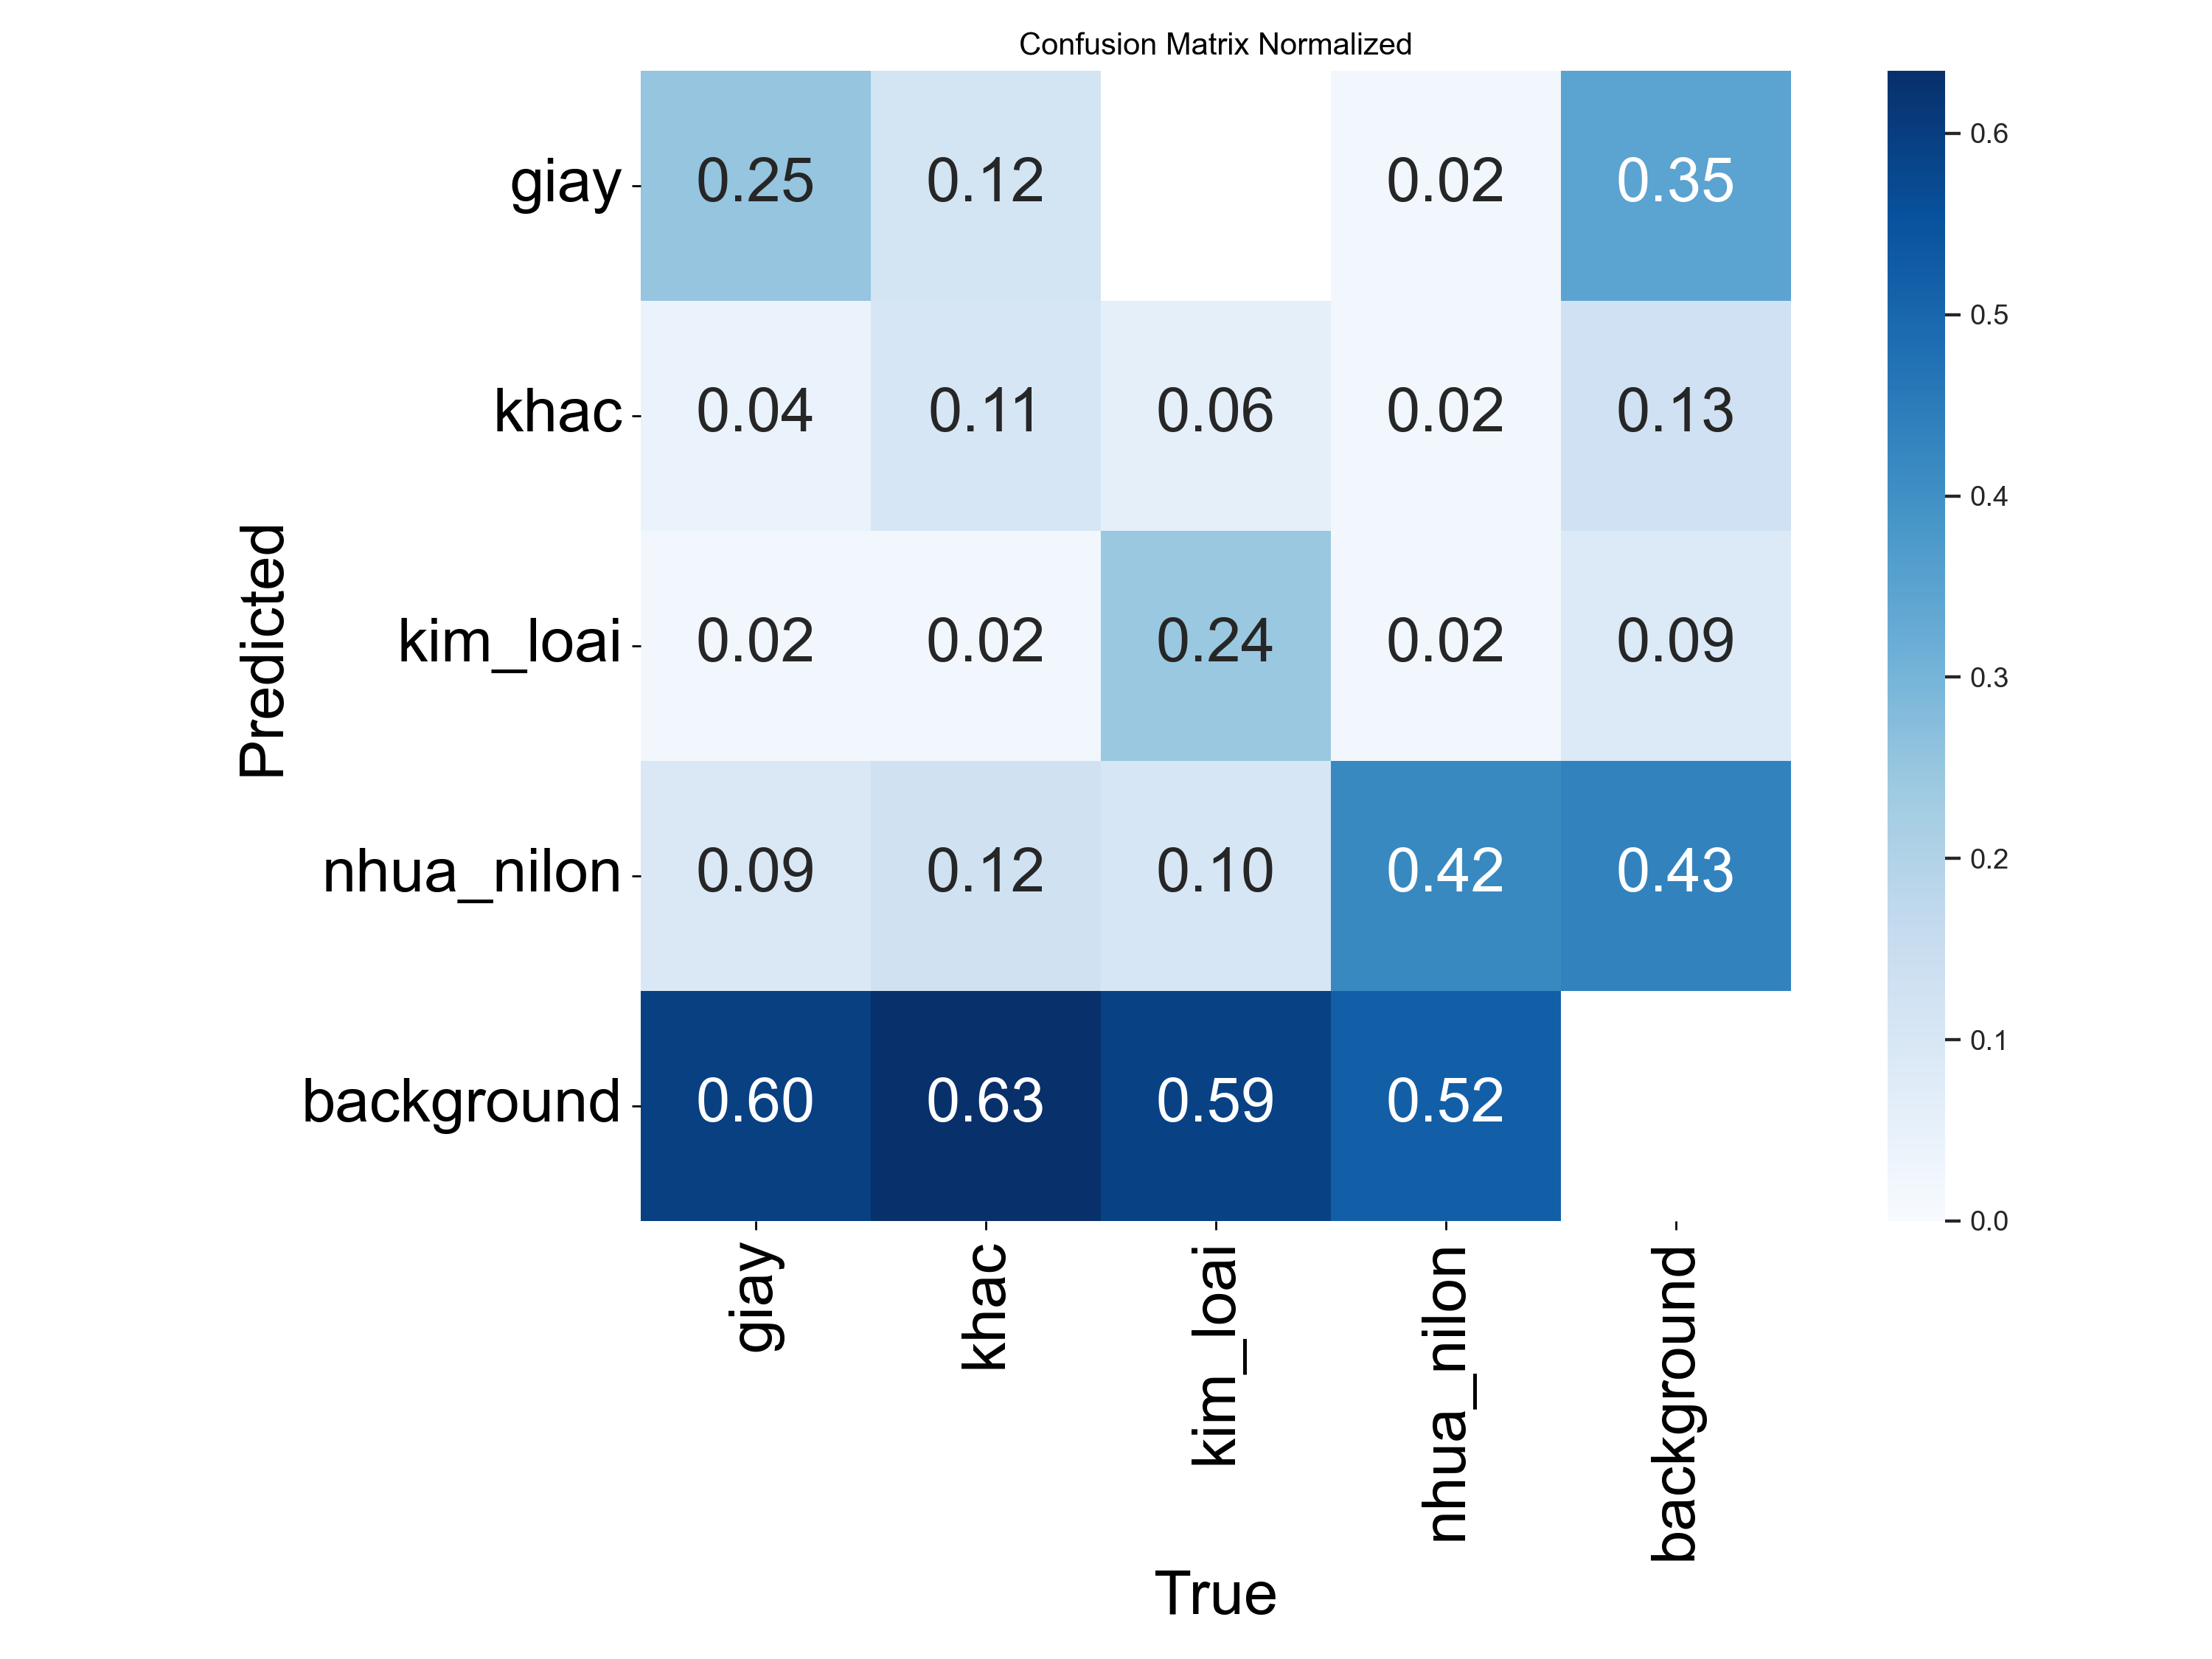
\includegraphics[width=0.9\textwidth]{matrix_tn2.png}
    \caption{Ma trận nhầm lẫn chuẩn hóa trên tập dữ liệu thử nghiệm của mô hình YOLOv8n trong việc phát hiện và phân loại rác}
    \label{fig:thucnghiem2.1}
\end{figure}

\section{Thực nghiệm 3 - Đánh giá mô hình dựa vào phát hiện và phân loại rác trên tập dữ liệu đã bổ sung ảnh nền không có nhãn}
 {\fontsize{13}{12} \selectfont

  Thực nghiệm 3 đối với tập xác thực không có sự chênh lệch đáng kể (Bảng \ref{tab:thucnghiem3.1}) so với kết quả của Thực nghiệm 2, tuy nhiên với tập dữ liệu thử nghiệm chỉ gồm các đối tượng ngoài tự nhiên thì mô hình
  cho thấy sự hiệu quả của việc bổ sung các hình ảnh nền giúp mô hình nhận dạng chính xác các lớp hơn, giảm việc bỏ sót hoặc nhận dạng nhầm thành các lớp khác (xem Hình \ref{fig:thucnghiem3.1}).
  Lớp "Kim loại", "Giấy" cho thấy sự cải thiện đáng kể, giảm bớt việc nhận dạng sai thành các lớp còn lại.
  Mô hình YOLOv8 vẫn đạt được kết quả tốt hơn trong việc huấn luyện, việc áp dụng các ảnh nền cũng tỏ ra hiệu quả hơn đối với mô hình YOLOv8n khi cải thiện được 5.8\% độ chính xác so với 1,1\% của mô hình YOLOv7-tiny.
  Hình \ref{fig:thucnghiem3.2} kết quả trong quá trình huấn luyện mô hình YOLOv8n.

 }

\begin{table}[h!]
    \centering
    \begin{threeparttable}
        \caption{Kết quả thực hiện Thực nghiệm 3 - đánh giá mô hình dựa vào phát hiện và phân loại rác trên tập dữ liệu đã bổ sung ảnh nền không có nhãn}

        \begin{tabular}{llrwr{2cm}rrr}
            \hline
            \multicolumn{1}{l}{\textbf{Tập dữ liệu}} & \textbf{Mô hình} & \multicolumn{1}{r}{\textbf{Kim loại}} & \multicolumn{1}{r}{\textbf{Giấy}} & \multicolumn{1}{r}{\textbf{Nhựa - nilon}} & \multicolumn{1}{r}{\textbf{Khác}} & \multicolumn{1}{r}{\textbf{Tất cả}} \\ \hline
            \multirow{2}{*}{Xác thực}                & YOLOv7-tiny      & 0,729                                 & 0,678                             & 0,546                                     & 0,477                             & 0,608                               \\ \cline{2-7}
                                                     & YOLOv8n          & \textbf{0,759}                        & \textbf{0,727}                    & \textbf{0,629}                            & \textbf{0,572}                    & \textbf{0,672}                      \\ \hline
            \multirow{2}{*}{Thử nghiệm}              & YOLOv7-tiny      & 0,445                                 & 0,393                             & 0,476                                     & 0,235                             & 0,387                               \\ \cline{2-7}
                                                     & YOLOv8n          & \textbf{0,514}                        & \textbf{0,451}                    & \textbf{0,556}                            & \textbf{0,263}                    & \textbf{0,446}                      \\ \hline
        \end{tabular}
        \label{tab:thucnghiem3.1}
    \end{threeparttable}
\end{table}

\begin{figure}[H]
    \centering
    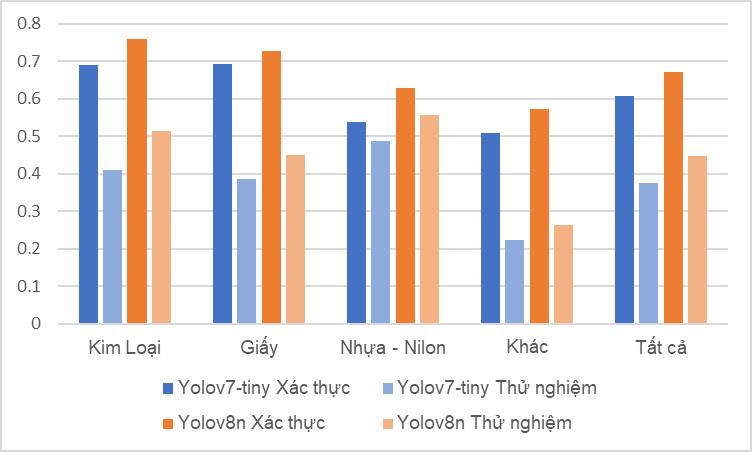
\includegraphics[width=0.8\textwidth]{thucnghiem3.1.jpg}
    \caption{Biểu đồ kết quả Thực nghiệm 3 - đánh giá mô hình dựa vào phát hiện và phân loại rác trên tập dữ liệu đã bổ sung ảnh nền không có nhãn}
    \label{fig:thucnghiem3}
\end{figure}

\begin{figure}[H]
    \centering
    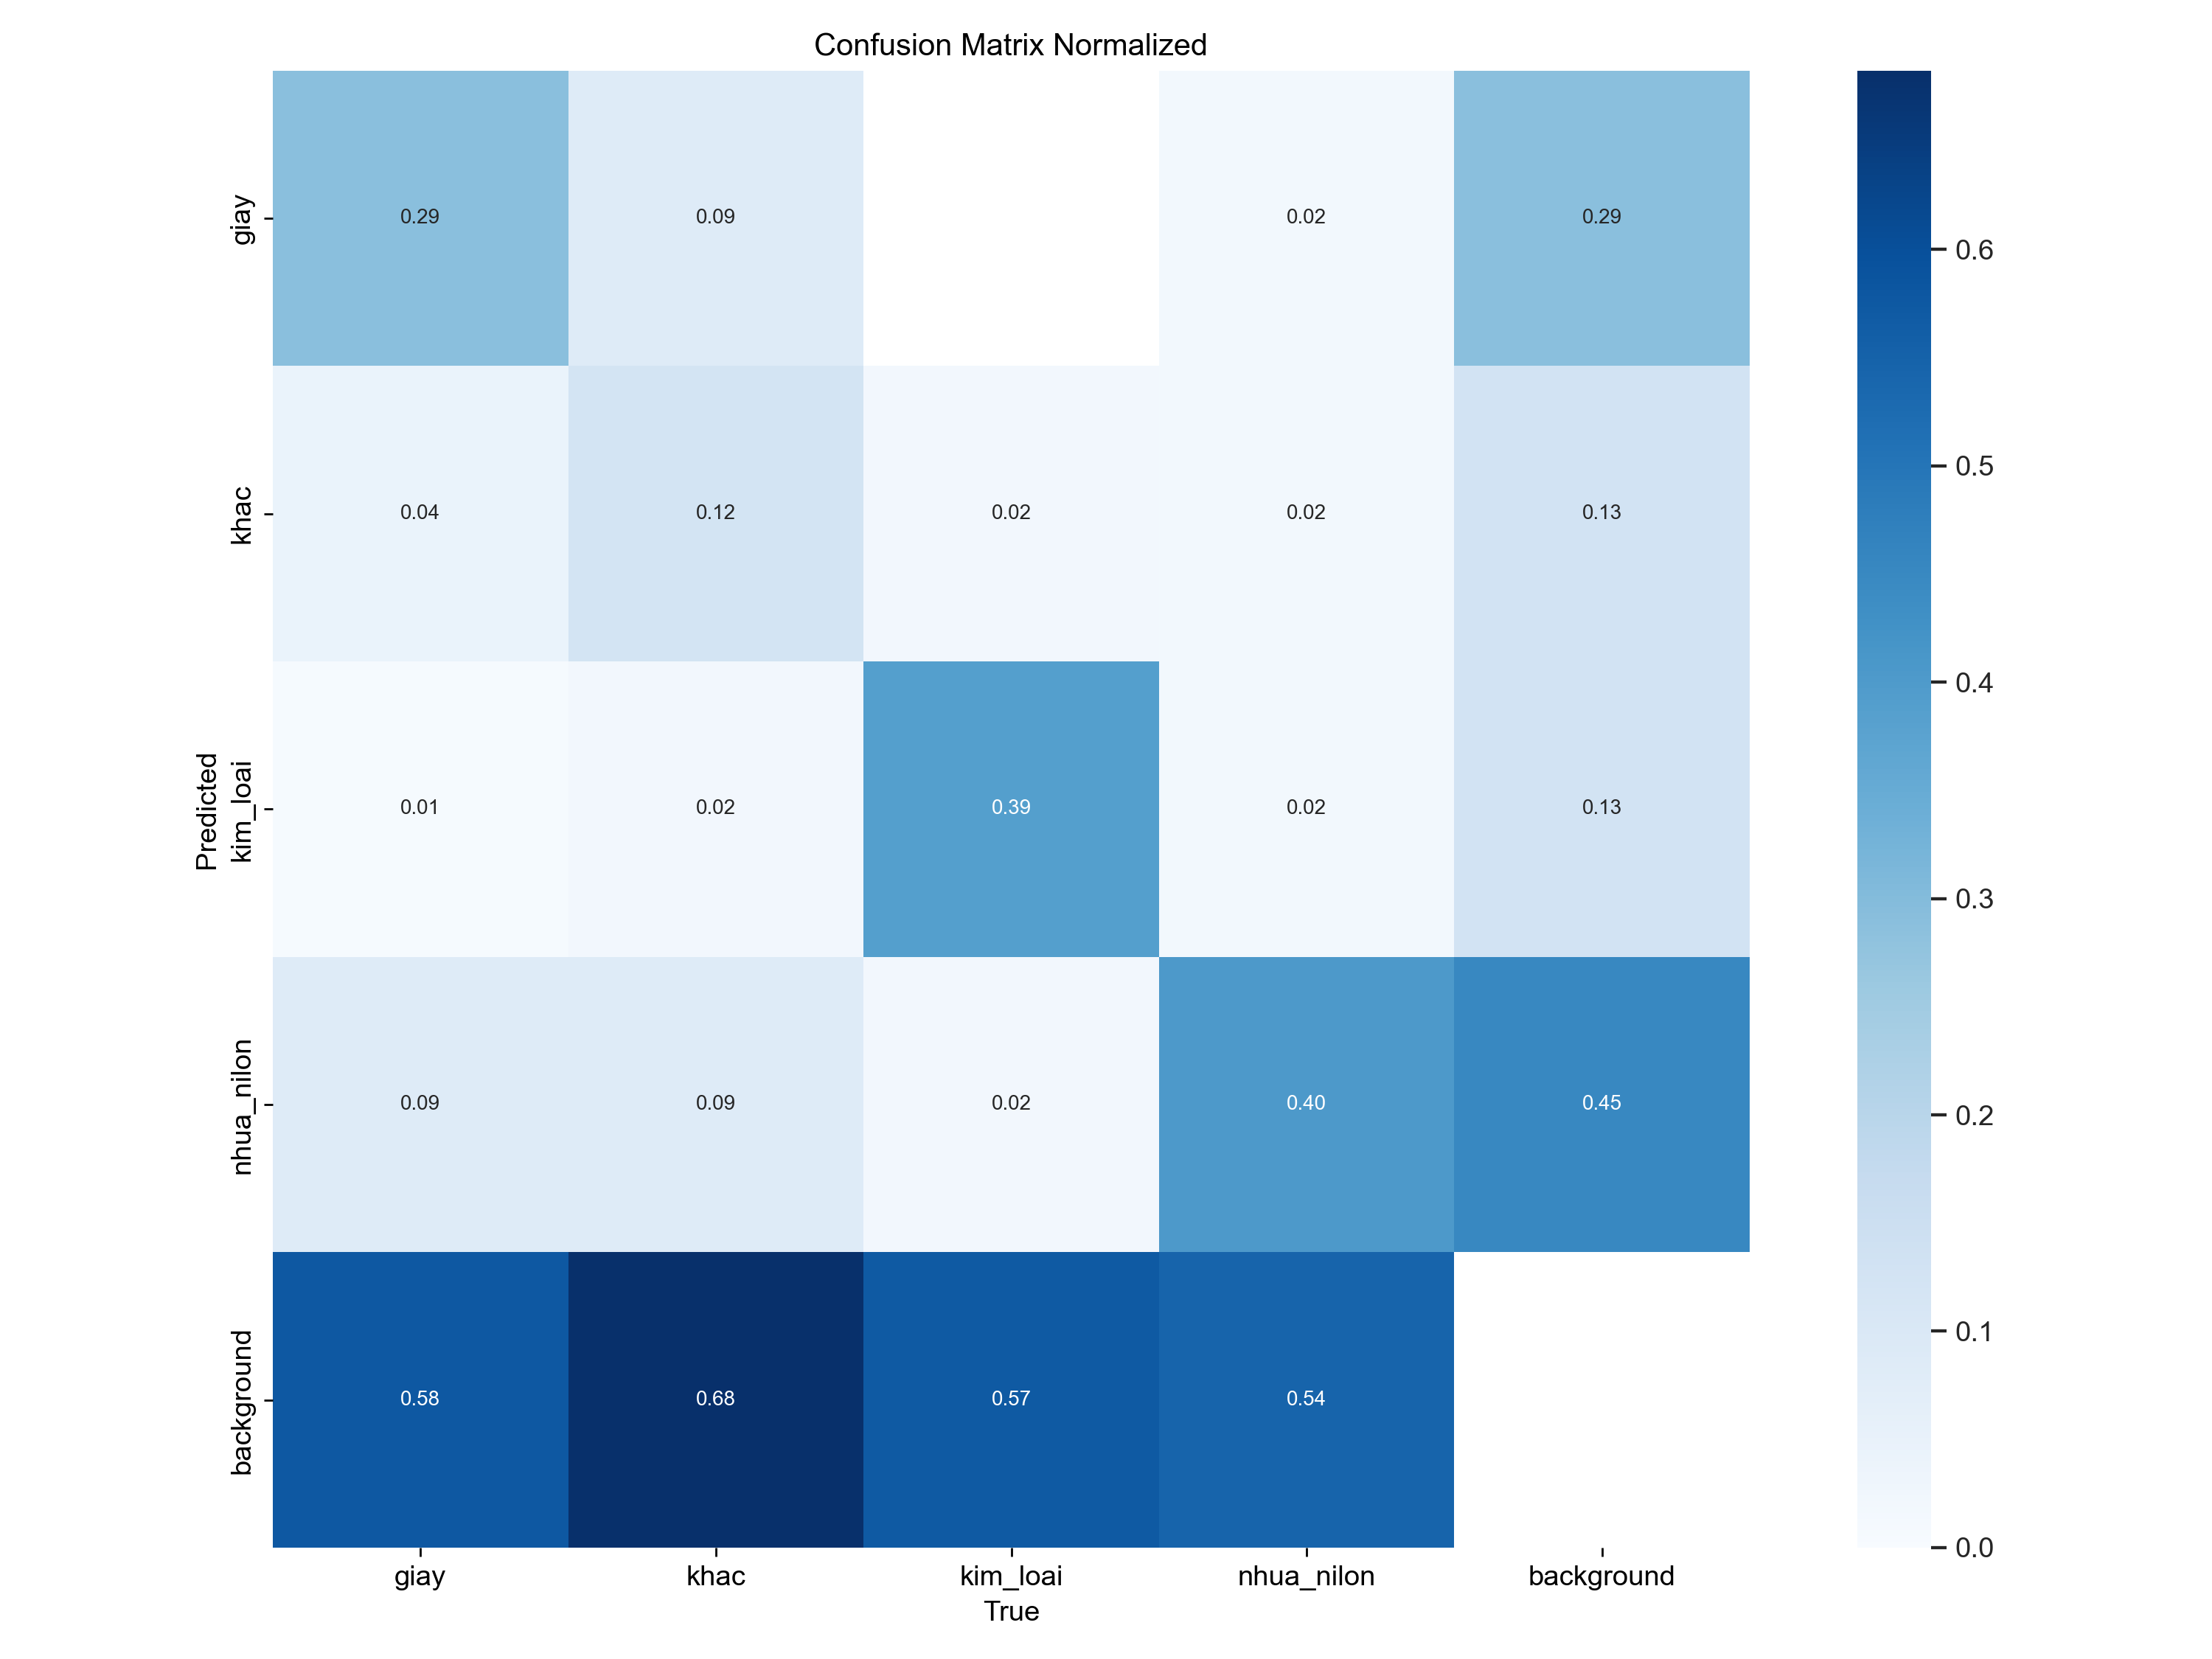
\includegraphics[width=1\textwidth]{matrix_tn3.png}
    \caption{Ma trận nhầm lẫn chuẩn hóa trên tập dữ liệu thử nghiệm mô hình YOLOv8n trọng việc phát hiện và phân loại rác khi bổ sung ảnh nền không có nhãn}
    \label{fig:thucnghiem3.1}
\end{figure}

\begin{figure}[H]
    \centering
    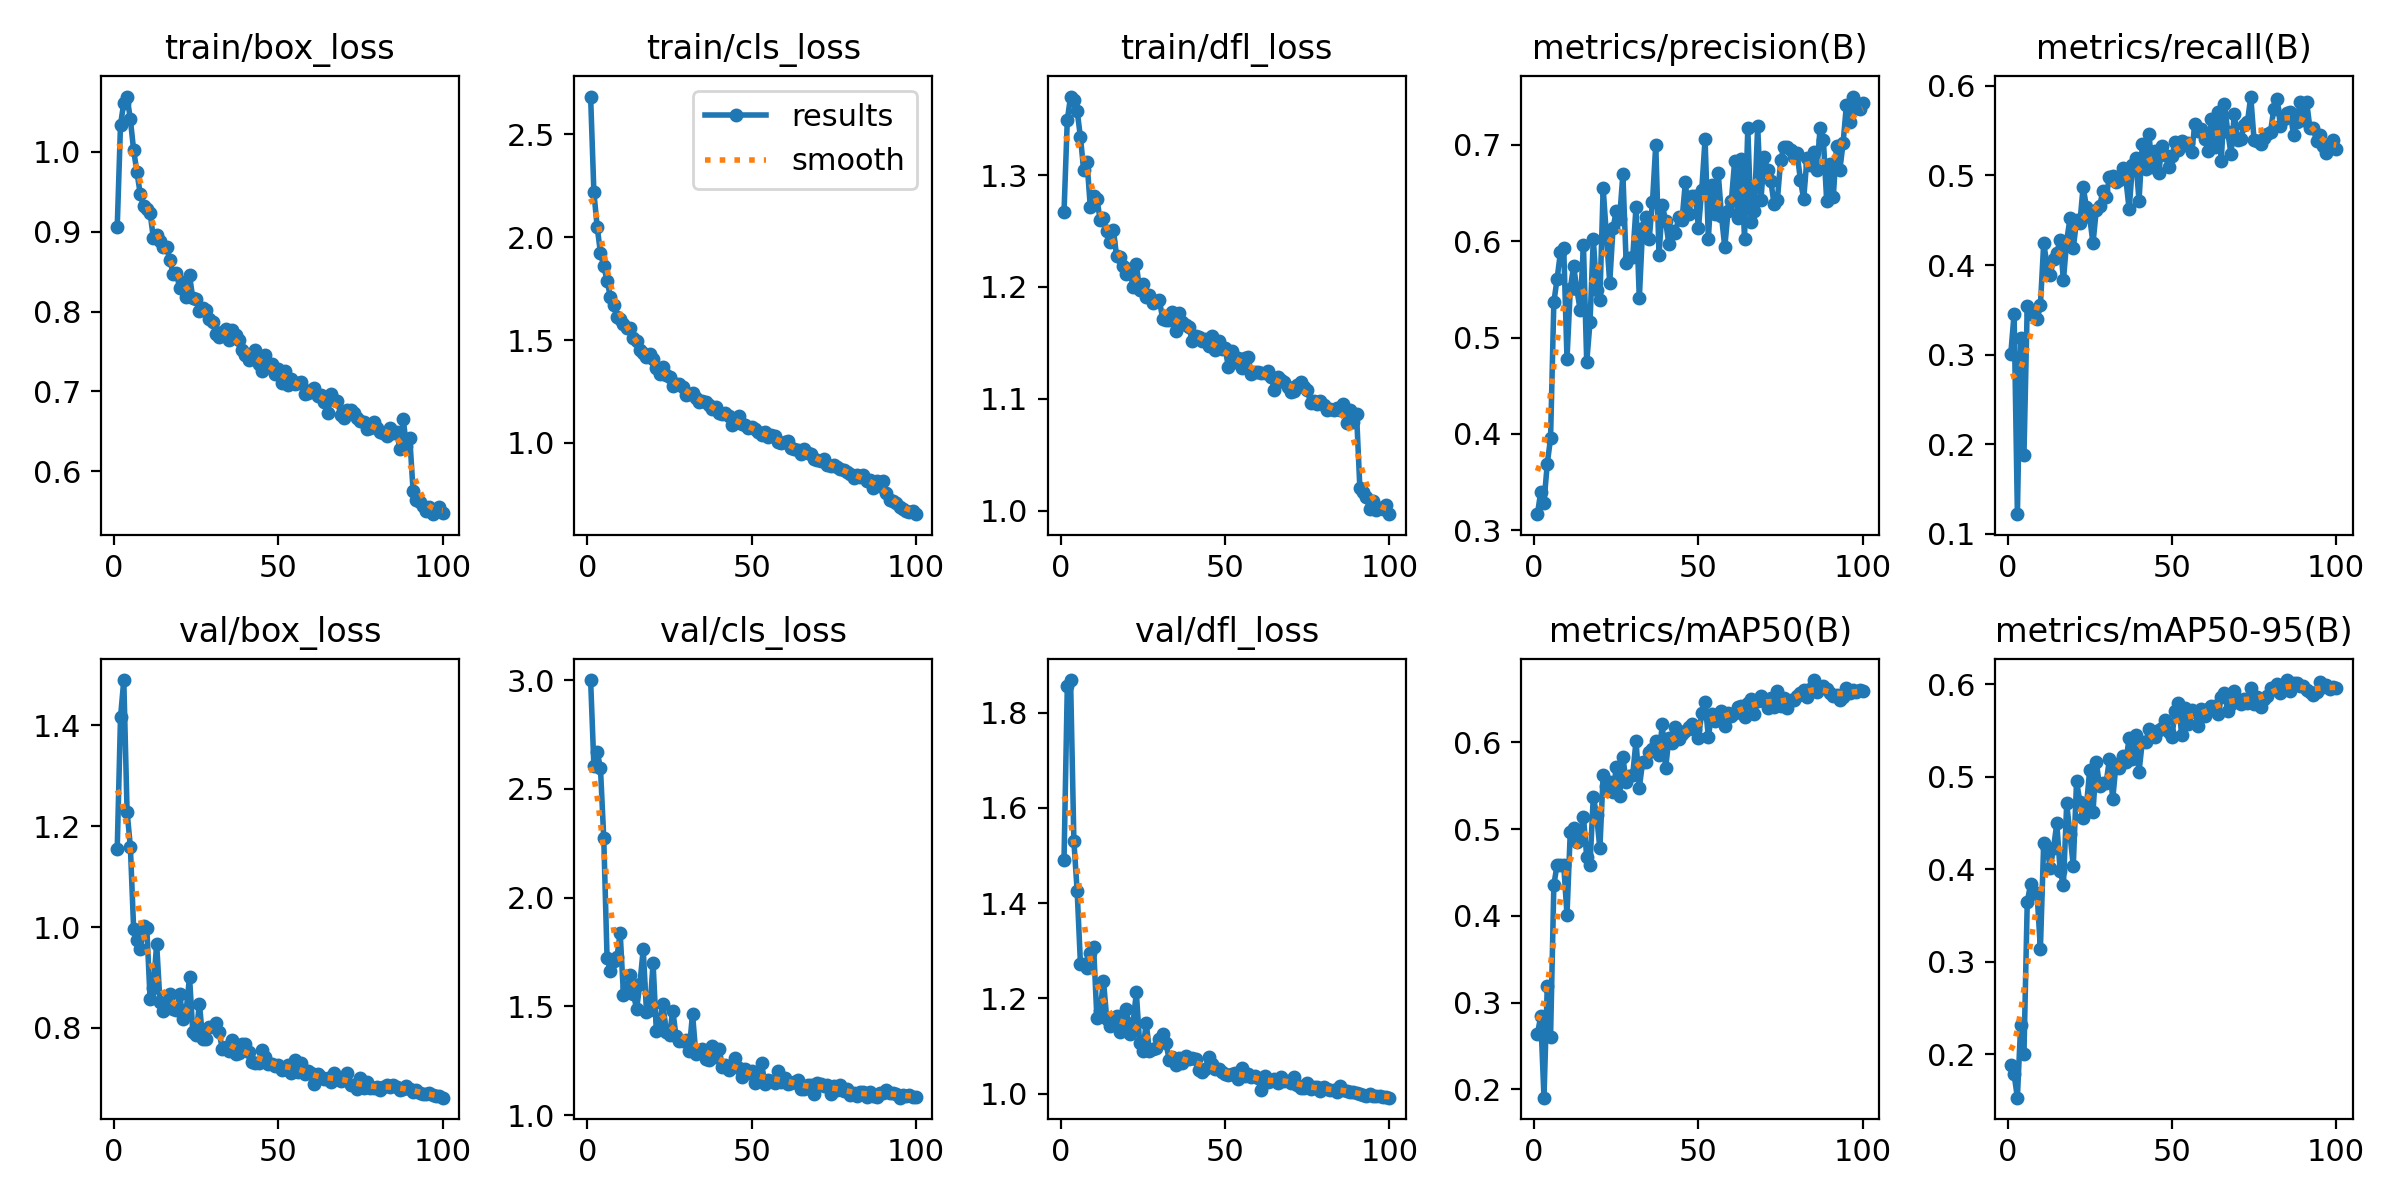
\includegraphics[width=1\textwidth]{results_yolo8.png}
    \caption{Các biểu đồ đánh giá của mô hình YOLOv8n}
    \label{fig:thucnghiem3.2}
\end{figure}


\section{Thảo luận}
 {\fontsize{13}{12} \selectfont

  Các kết quả được so sánh cho ta thấy cùng một kết quả: mô hình YOLOv8 hoạt động tốt hơn hai mô hình còn lại.
  Từ đánh giá việc phát hiện đối tượng (phát hiện một lớp) đến việc phát hiện và phân loại rác thành bốn lớp theo thành phần.
  Các mô hình luôn gặp khó khăn khi phát hiện đối tượng với lớp rác khác vì có kích thước nhỏ và tính đa dạng.
  Điều đó cho thấy việc gán nhãn và định nghĩa các rác cụ thể thành các lớp đặc trưng mang ý nghĩa quan trọng,
  tương tự như việc chuyển đổi các lớp ở dữ liệu TACO thành các lớp ở dữ liệu nghiên cứu.
  Thực nghiệm 3 bổ sung thêm dữ liệu từ các nền đã tăng độ chính xác của mô hình được mô tả chi tiết ở Bảng \ref{tab:thaoluan1} và Hình \ref{fig:final}.

 }


\begin{table}[h!]
    \centering
    \begin{threeparttable}
        \caption{Kết quả thể hiện độ cải thiện của mô hình YOLOv8 khi bổ sung ảnh nền}
        \begin{tabular}{lrrrrr}
            \hline
            \multicolumn{1}{l}{\textbf{\#}} & \textbf{Kim Loại} & \textbf{Giấy} & \textbf{Nhựa - Nilon} & \textbf{Khác} & \textbf{Tất cả} \\ \hline
            Tập dữ liệu                     & 0,377             & 0,415         & 0,553                 & 0,207         & 0,388           \\ \hline
            Tập bổ sung nền                 & 0,514             & 0,451         & 0,556                 & 0,263         & 0,446           \\ \hline
            Độ cải thiện                    & +0,13             & +0,036        & +0,003                & +0,056        & +0,058          \\ \hline
        \end{tabular}
        \label{tab:thaoluan1}
    \end{threeparttable}
\end{table}


{\fontsize{13}{12} \selectfont

Bảng \ref{tab:related}
mô tả các nghiên cứu liên quan ở mục \ref{sec:nnlq} và kết quả đạt được của nghiên cứu hiện tại với các thông tin về tập dữ liệu, số lớp của mô hình, mô hình sử dụng, loại nhận dạng và kết quả đạt được dựa trên đánh giá từng nghiên cứu.
Nhìn chung các nghiên cứu đạt kết quả không cao đối với nhiệm vụ phát hiện hoặc phân đoạn đối tượng, điều đó cho thấy việc khó khăn khi áp dụng các dữ liệu ngoài tự nhiên vì nhiều dữ liệu gây nhiễu, khó khăn trong việc gán nhãn.
Nghiên cứu của chúng tôi bước đầu cho thấy kết quả khả quan đối với nhiệm vụ phát hiện và phân loại rác theo thành phần. Đối với nhiệm vụ chỉ phát hiện rác nghiên cứu cho thấy kết quả tốt hơn so với nghiên cứu của tác giả TACO \cite{proença2020taco} và Sylwia \cite{Majchrowska_2022}.
Đối với nhiệm vụ phân loại, mô hình đạt kết quả tương đối khi so với nghiên cứu của Carolis \cite{9122693} vì phân loại rác theo thành phần mang tính khái quát, trong từng loại rác không có hình dạng, màu sắc đặc trưng.
Nghiên cứu cũng đã thử nghiệm kết quả với 100 hình ảnh của tập dữ liệu RealWaste \cite{info14120633} được lấy mẫu trực tiếp từ các thùng rác đô thị, bộ dữ liệu là bản nâng cấp của TrashNet khi các vật phẩm rác đã bị biến dạng vì vùi lắp. 
Các hình ảnh trong RealWaste được chụp trong môi trường trong nhà có nền khác nhau, nghiên cứu đạt được kết quả là 67,2\%, trong đó cao nhất là lớp "Kim loại" với 81,5\% và thấp nhất là lớp "Khác" với 40,1\% (xem Hình \ref{fig:realwaste}).
Điều này cho thấy mô hình có thể thực hiện trên tập dữ liệu đa dạng với môi trường khác nhau.

}

\bigskip

{\fontsize{13}{12} \selectfont
Ý tưởng phân loại rác thành bốn lớp của nghiên cứu dựa vào số lớp của các nghiên cứu phân lớp và tình hình thực tế sau khi thu thập dữ liệu ở địa phương. Kết hợp từ việc lấy ý tưởng từ các tập dữ liệu có sẵn và huấn luyện trên các mô hình gần đây,
nghiên cứu cho thấy sự cải thiện kết quả so với các nghiên cứu phân đoạn hay phát hiện đối tượng trên tập dữ liệu về rác.

}

\begin{figure}[H]
    \centering
    \subfloat[\centering {\fontsize{11}{10} \selectfont Hình ảnh của tập dữ liệu được gán nhãn }]{{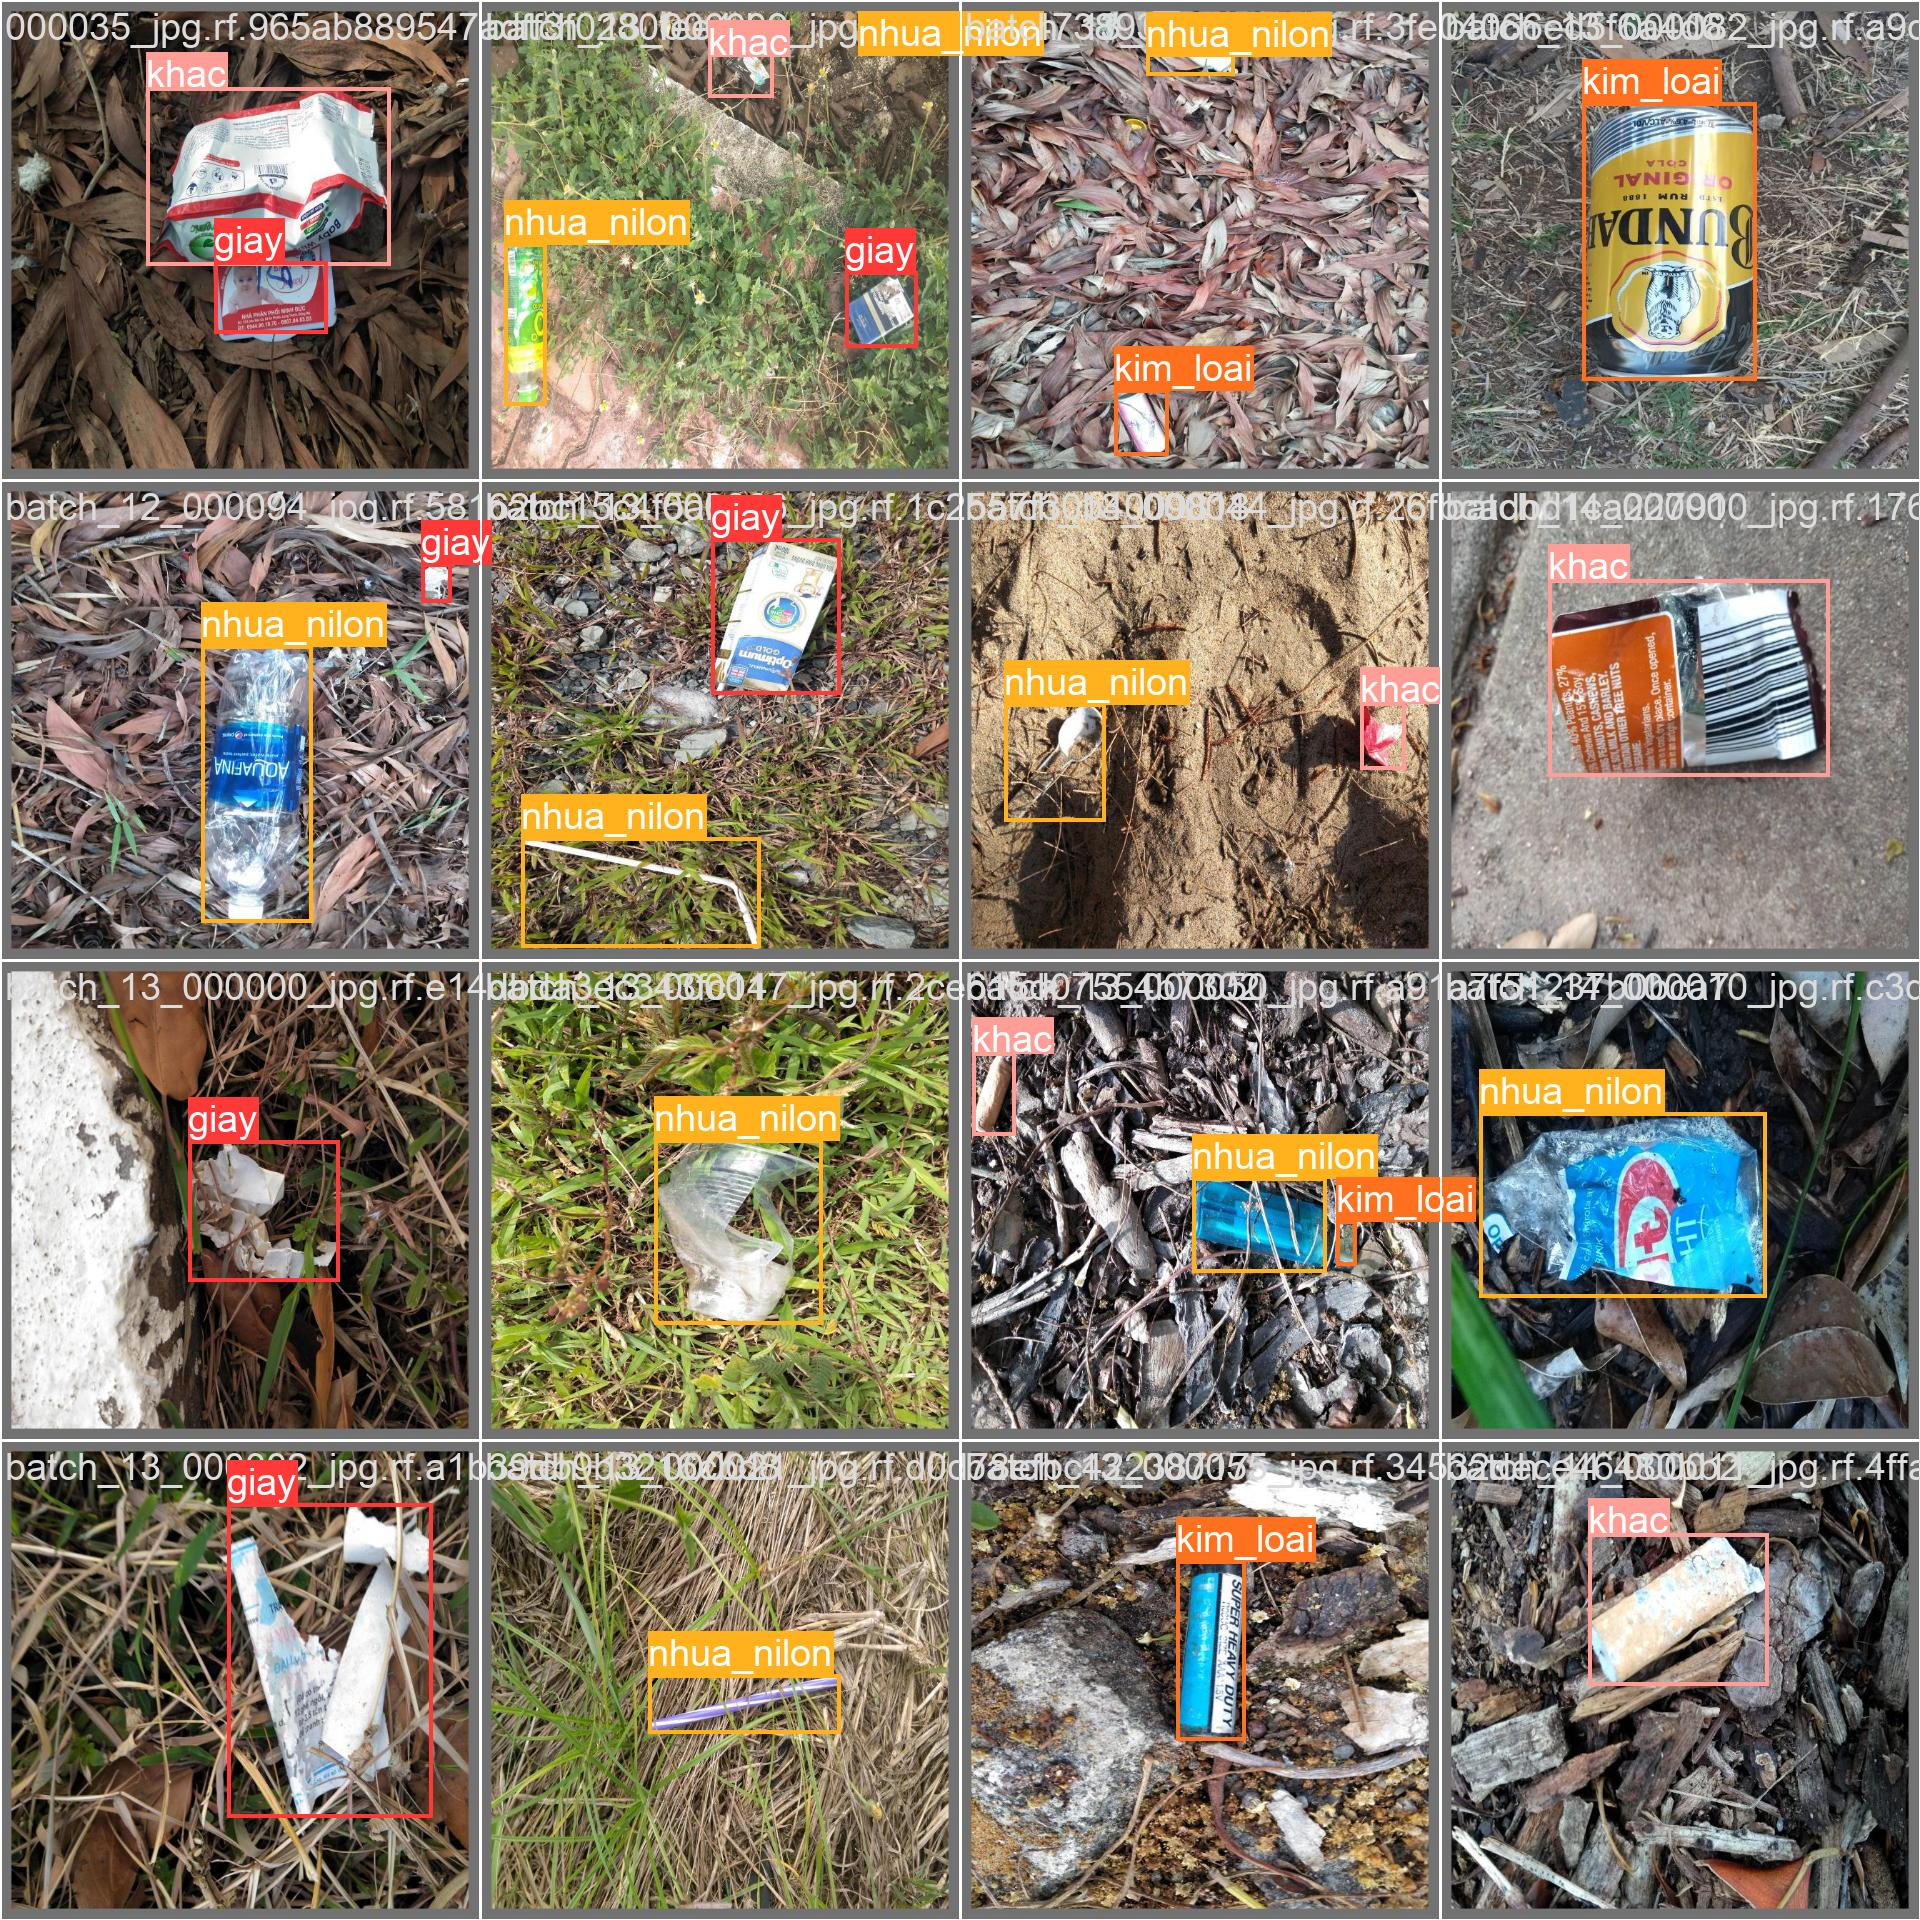
\includegraphics[width=10cm]{yolov8_label.jpg} \label{fig:yolov8_label}}}%
    \qquad
    \subfloat[\centering {\fontsize{11}{10} \selectfont Hình ảnh phát hiện khi chưa tăng cường ảnh nền}]{{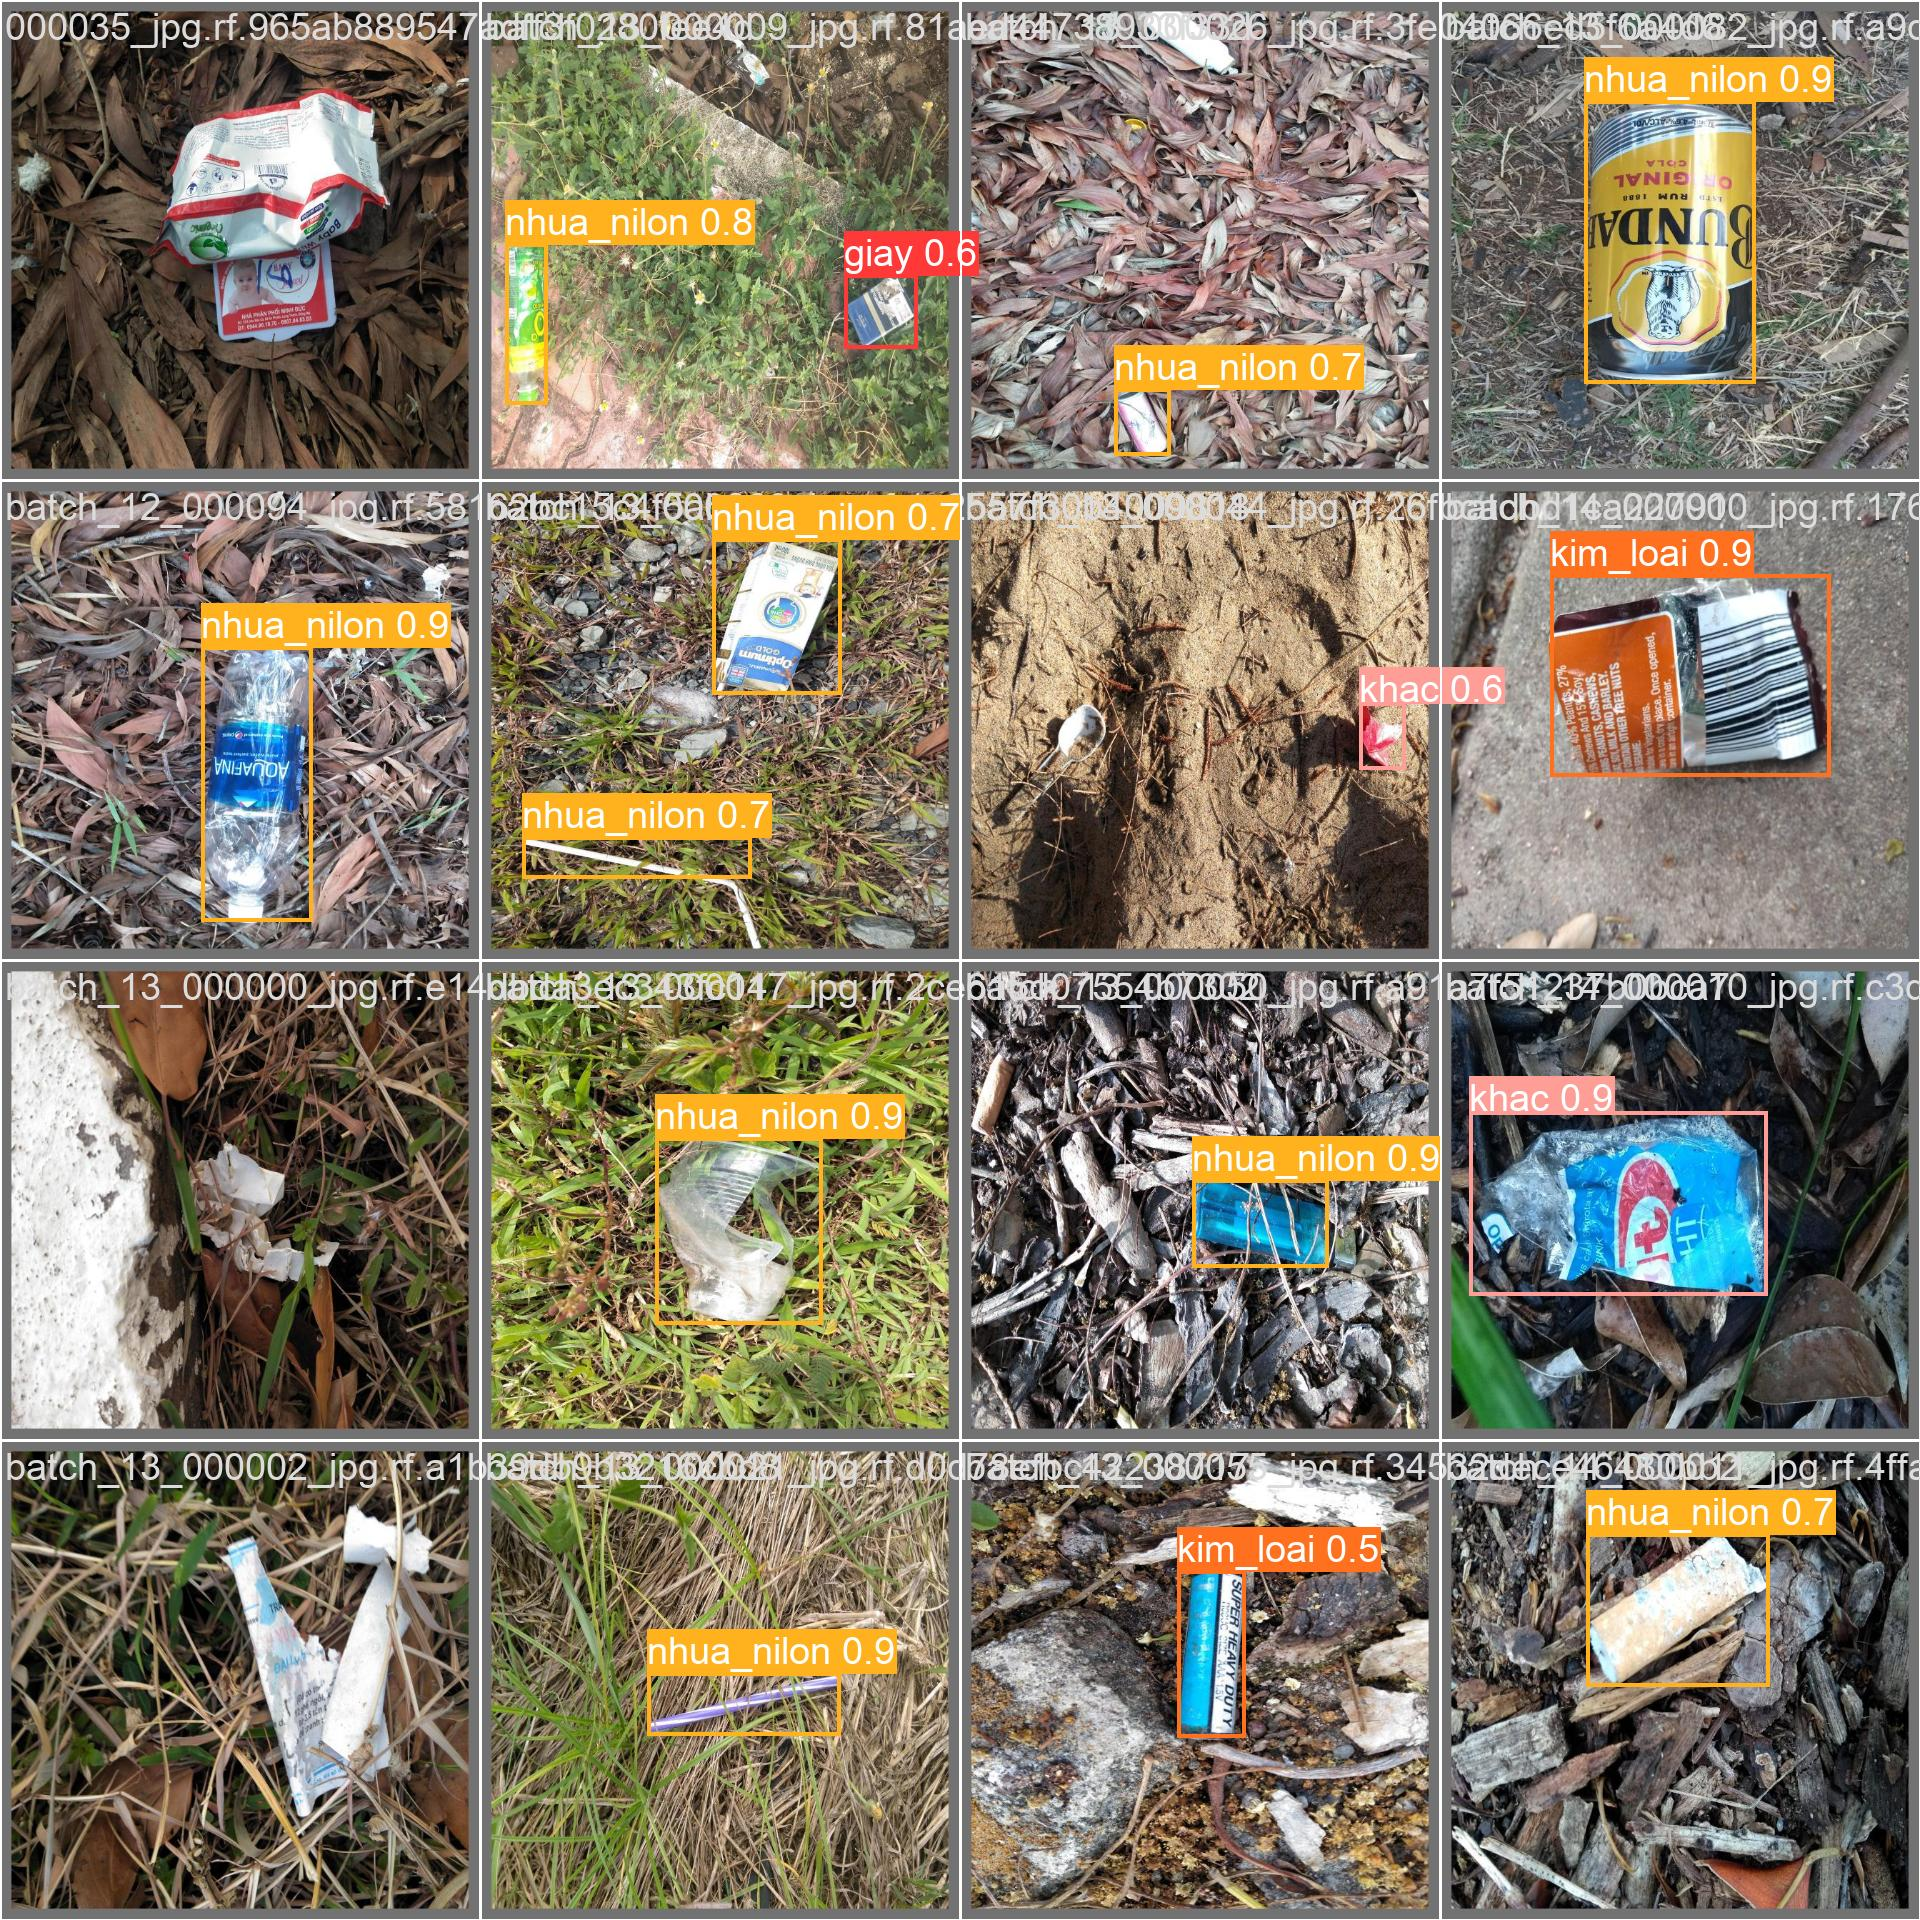
\includegraphics[width=7cm]{yolov8_pred_nobg.jpg} \label{fig:yolov8_pred_nobg}}}%
    \qquad
    \subfloat[\centering {\fontsize{11}{10} \selectfont Hình ảnh phát hiện khi tăng cường ảnh nền}]{{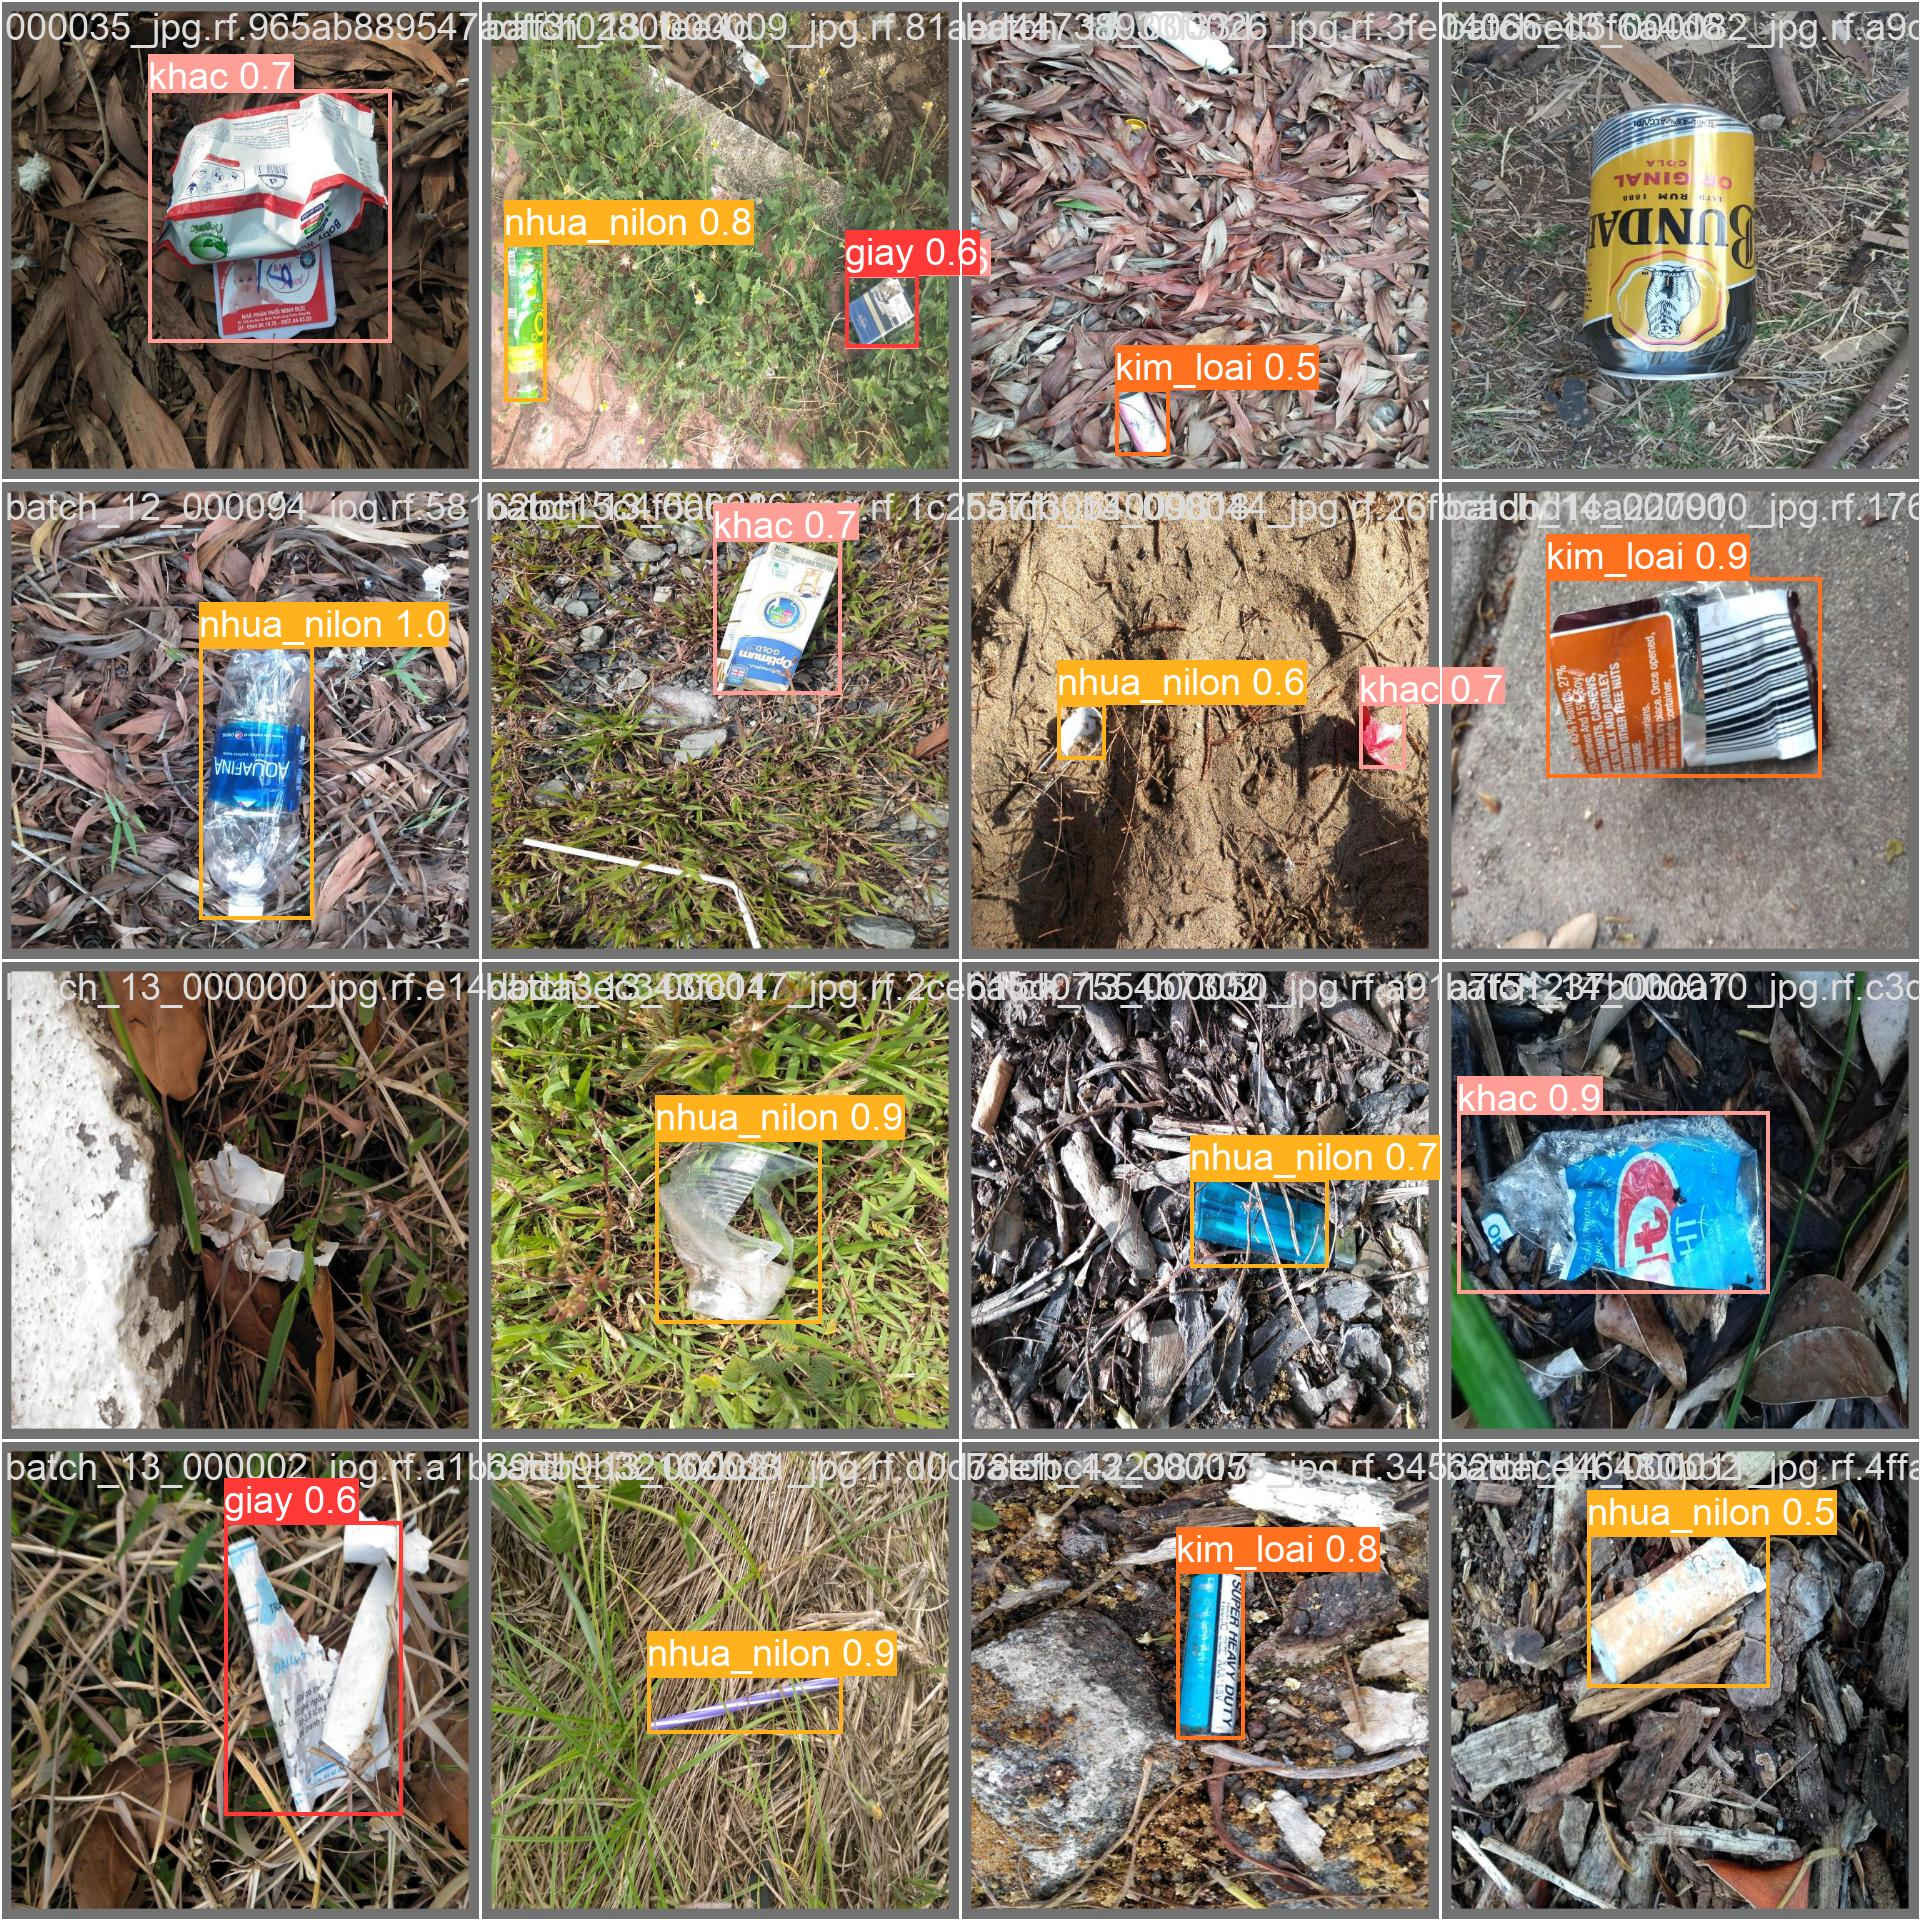
\includegraphics[width=7cm]{yolov8_pred.jpg} \label{fig:yolov8_pred}}}%
    \caption{Hình ảnh so sánh kết quả phát hiện và phân loại rác khi tăng cường dữ liệu}
    \label{fig:final}
\end{figure}


\begin{figure}[H]
    \centering
    \includegraphics[width=1\textwidth]{realwaste_test.png}
    \caption{Hình ảnh mô hình nhận dạng trên tập dữ liệu RealWaste}
    \label{fig:realwaste}
\end{figure}

{\fontsize{13}{12} \selectfont

Tuy nhiên nghiên cứu đạt kết quả không cao, mô hình gặp khó khăn với các đối tượng nhỏ, đối tượng bị che khuất hoặc khó nhận thấy vì ẩn vào nền như Hình \ref{fig:sai1}.
Mô hình cũng dễ nhầm lẫn giữa các lớp với nhau vì tập dữ liệu còn ít, Hình \ref{fig:sai2} cho thấy vỏ lon thuộc lớp "Kim loại" nhưng nhận dạng sai thành rác "Khác".
Các đối tượng ngoài tự nhiên như cây, đá cũng dễ nhận dạng nhầm thành rác hoặc các hộp giới hạn bao không hết đối tượng như Hình \ref{fig:sai3}.
Hơn nữa, mô hình cũng xảy ra tình trạng chồng chéo các hộp giới hạn, làm cho một đối tượng có nhiều lớp (xem Hình \ref{fig:sai4}).

}


\begin{figure}[H]
    \centering
    \subfloat[\centering {\fontsize{11}{10} \selectfont Bỏ qua không phát hiện đối tượng }]{{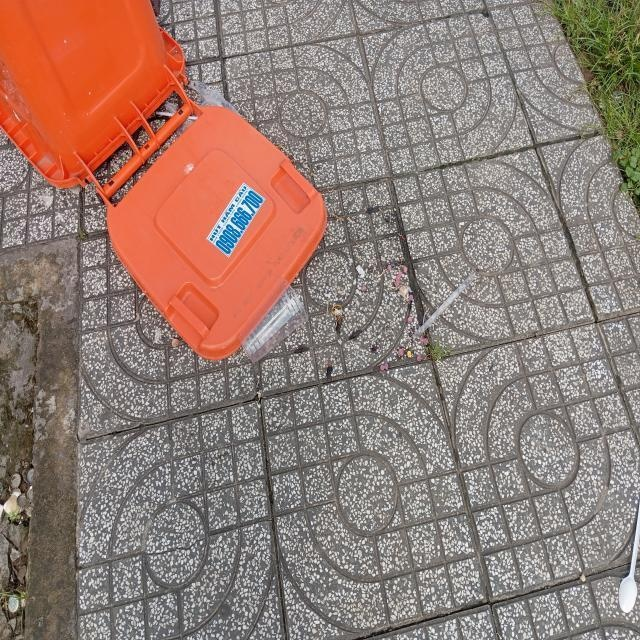
\includegraphics[width=7cm]{result_sai2.jpg} \label{fig:sai1}}}%
    \qquad
    \subfloat[\centering {\fontsize{11}{10} \selectfont Phân loại không đúng}]{{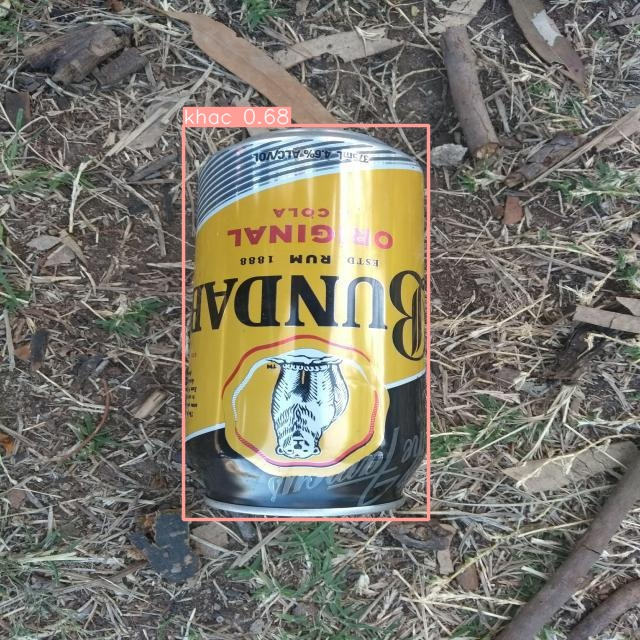
\includegraphics[width=7cm]{result_sai4.jpg} \label{fig:sai2}}}%
    \qquad
    \subfloat[\centering {\fontsize{11}{10} \selectfont Phát hiện dư và hộp không bao hết đối tượng}]{{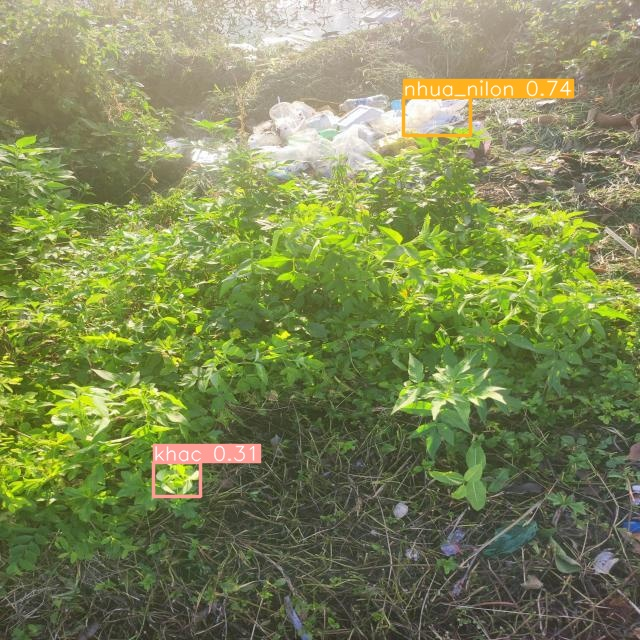
\includegraphics[width=7cm]{result_sai1.jpg} \label{fig:sai3}}}%
    \qquad
    \subfloat[\centering {\fontsize{11}{10} \selectfont Nhiều hộp cho một đối tượng, đối tượng có nhiều lớp}]{{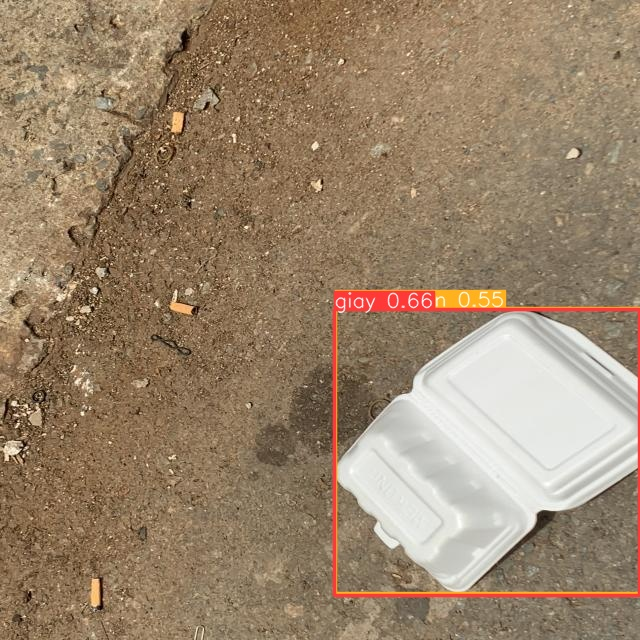
\includegraphics[width=7cm]{result_sai3.jpg} \label{fig:sai4}}}%
    \caption{Hình ảnh mô hình nhận dạng sai với các đối tượng ngoài tự nhiên}
    \label{fig:sai}
\end{figure}


\begin{table*}[ht!]

    \begin{threeparttable}
        \caption{Mô tả các nghiên cứu liên quan ở mục \ref{sec:nnlq} và kết quả của đề tài}
        % \begin{tabularx}{\columnwidth}{|X|X|c|X|X|}
        \begin{tabularx}{\columnwidth}{sbsbbb}
            \hline
            \textbf{\#}
                                                            & \textbf{Dữ liệu \newline (\# ảnh)}
                                                            & \textbf{Số \newline lớp}
                                                            & \textbf{Mô hình}
                                                            & \textbf{Loại\newline nhận dạng}
                                                            & \textbf{Kết quả của nghiên cứu}
            \\ \hline

            Yang, Thung \etal \cite{yang2016classification} &
            TrashNet
                                                            & 6
                                                            & SVM \newline CNN
                                                            & Phân lớp
                                                            & Độ chính xác: 63\%                                              \\ \hline

            Jash và Sagar \etal \cite{shah2022method}
                                                            & 25.077
                                                            & 2
                                                            & SVM \newline CNN
                                                            & Phân lớp
                                                            & Độ chính xác: 94,96\%                                           \\ \hline

            Carolis \etal \cite{9122693}
                                                            & 2.714
                                                            & 4
                                                            & YOLOv3
                                                            & Phát hiện
                                                            & mAP50: 59,59\%                                                  \\ \hline


            Proença \etal \cite{proença2020taco}
                                                            & TACO
                                                            & 1, 10
                                                            & Mask RCNN
                                                            & Phân đoạn
                                                            & 1 lớp mAP: 15,9\% \newline 10 lớp: 17,6\%                       \\ \hline

            Fulton \etal \cite{8793975}
                                                            & Trash-ICRA19
                                                            & 3
                                                            & YOLOv2 \newline SSD \newline FasterRCNN
                                                            & Phát hiện
                                                            & YOLOv2 47,9\%  \newline SSD: 67,4\%  \newline Faster RCNN: 81\% \\ \hline

            Sylwia \etal  \cite{Majchrowska_2022}
                                                            & detect waste + \newline (Gồm TACO)
                                                            & 1, 7
                                                            & EfficientNet-B2
                                                            & Phát hiện
                                                            & 1 lớp-mAP50: 46,9\% \newline 7 lớp-mAP50: 11,9\%                \\ \hline

            Nghiên cứu này
                                                            & khoảng 4.000
                                                            & 1, 4
                                                            & YOLOv8n
                                                            & Phát hiện
                                                            & 1 lớp-mAP50: 73\% \newline 4 lớp-mAP50: 44,6\%                  \\ \hline
        \end{tabularx}
        \label{tab:related}
    \end{threeparttable}

\end{table*}

\bigskip
{\fontsize{13}{12} \selectfont

    Tổng kết lại, nghiên cứu đã cho thấy mô hình YOLOv8 có hiệu suất vượt trội ở độ chính xác
    mà còn có số lượng tham số ít hơn giúp việc huấn luyện nhanh, phù hợp với việc cải thiện độ chính xác của mô hình khi dữ liệu được tăng cường.
    Nghiên cứu cho thấy tầm quan trọng của việc kết hợp dữ liệu, gán nhãn phân loại và áp dụng các hình không có đối tượng giúp cải thiện hiệu suất của mô hình khi thực nghiệm ngoài tự nhiên.
    Tuy nhiên để xây dựng hệ thống cần xử lý việc đối tượng có nhiều nhãn bằng cách so khớp vị trí tọa độ, diện tích và lấy độ tin cậy của hộp có điểm cao nhất.
}

\section{Bản đồ phân bố rác thải ở ĐBSCL}
{\fontsize{13}{12} \selectfont 

Nghiên cứu đã xây dựng hệ thống nhận đầu vào là hình ảnh rác được thu thập trên đường phố với các tùy chọn mô hình và video (xem Hình \ref{fig:demo1.1}). 
Hình ảnh sau đó được thay đổi kích thước thành ảnh 640x640 và tiến hành phân loại, sau đó trả kết quả cho người dùng nếu hình ảnh hợp lệ (xem Hình \ref{fig:demo1})
Sau khi phân loại, hình ảnh, nhãn và hộp giới hạn sẽ được lưu trữ trong CSDL MongoDB để hiển thị các thông tin cần thiết lên bản đồ (xem Hình \ref{fig:demo1.2}).
Hiện tại hệ thống chỉ ghi nhận lưu trữ hình ảnh khi chọn mô hình YOLOv8 cho việc phân loại bốn lớp và hình ảnh có thông tin về tọa độ vị trí.

}

\begin{figure}[H]
    \centering
    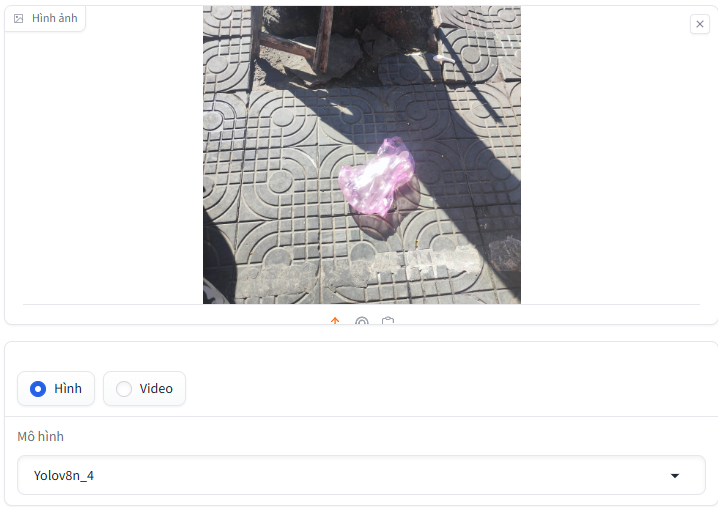
\includegraphics[width=1\textwidth]{demo1.1.png}
    \caption{Hệ thống nhận hình ảnh là rác được chụp trên đường phố}
    \label{fig:demo1.1}
\end{figure}

\begin{figure}[H]
    \centering
    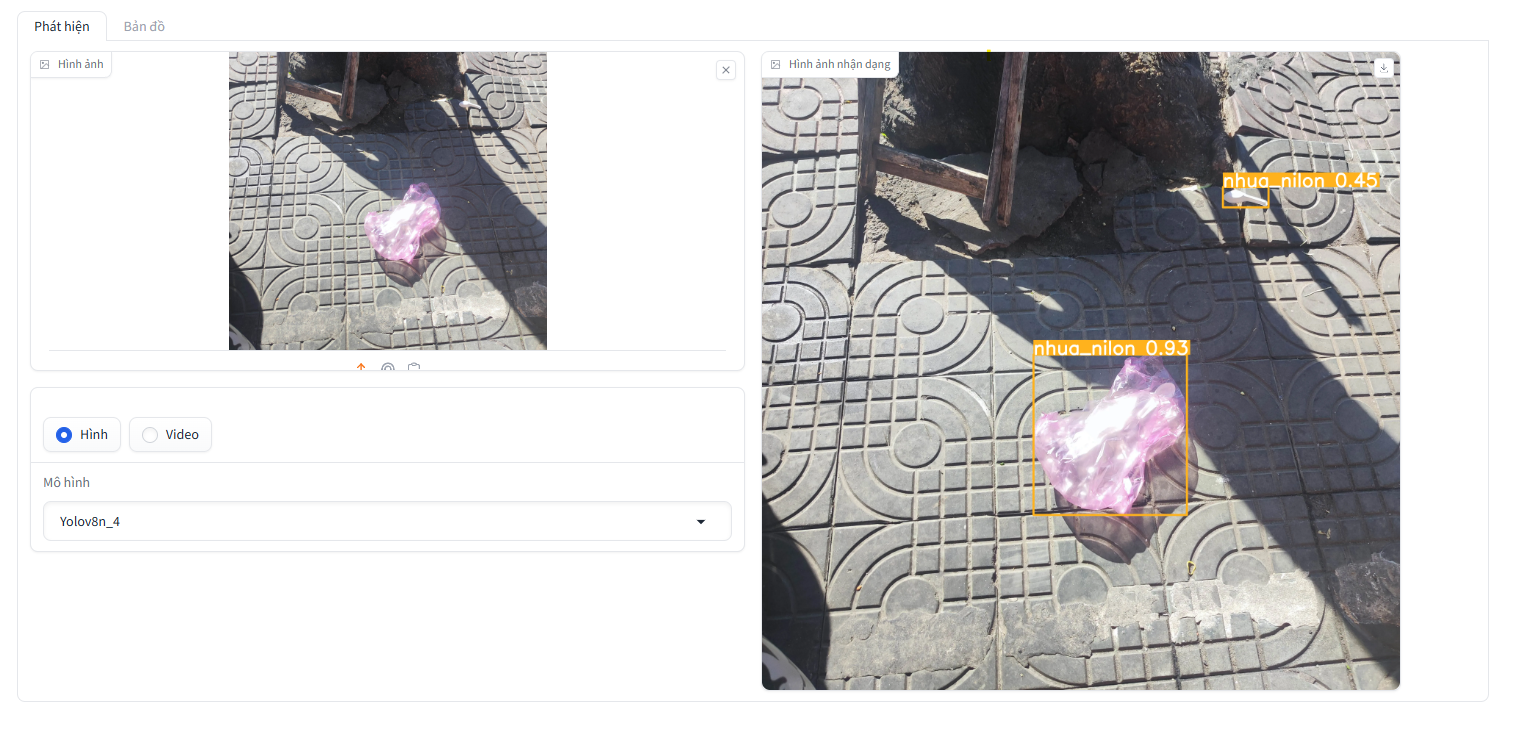
\includegraphics[width=1\textwidth]{demo1.png}
    \caption{Hệ thống tiến hành phân loại rác theo thành phần và hiển thị hình ảnh kết quả}
    \label{fig:demo1}
\end{figure}

\begin{figure}[H]
    \centering
    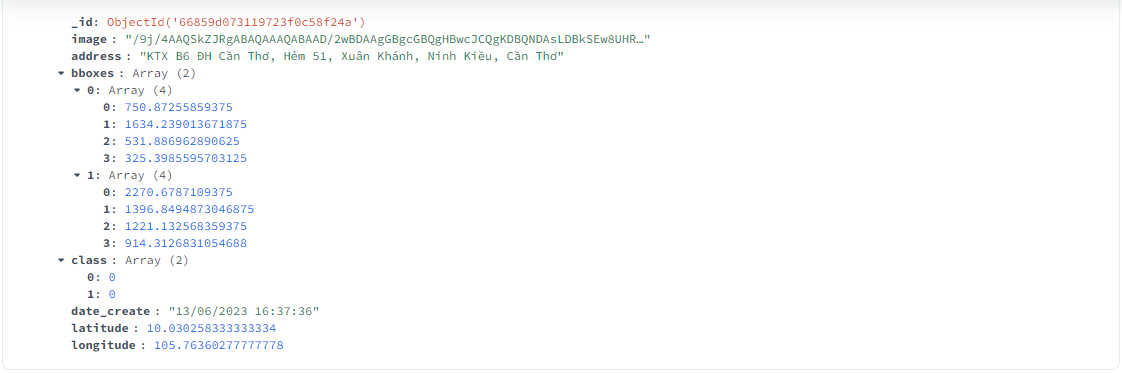
\includegraphics[width=1\textwidth]{demo1.2.png}
    \caption{Các thông tin được lưu trữ trong CSDL của hệ thống gồm hình, địa chỉ, hộp, lớp, ngày tạo và tọa độ}
    \label{fig:demo1.2}
\end{figure}

{\fontsize{13}{12} \selectfont 

Bản đồ phân bố cung cấp thông tin về mật độ phân bố của từng loại rác ở mỗi khu vực, dữ liệu được hiển thị ở ba tỉnh Vĩnh Long, Cần Thơ, Trà Vinh như Hình \ref{fig:demo2}. 
Có hai tùy chọn để hiển thị là thông tin về loại rác và loại bản đồ. Người dùng có thể chọn và bỏ chọn để lọc ra các loại rác cần hiển thị, mặc định hệ thống sẽ chọn tất cả bốn loại. 
Ngoài ra có thể chọn loại bản đồ là thông tin vị trí hoặc bản đồ nhiệt tùy theo mục đích sử dụng (xem Hình \ref{fig:demo2.1}).

}

\begin{figure}[H]
    \centering
    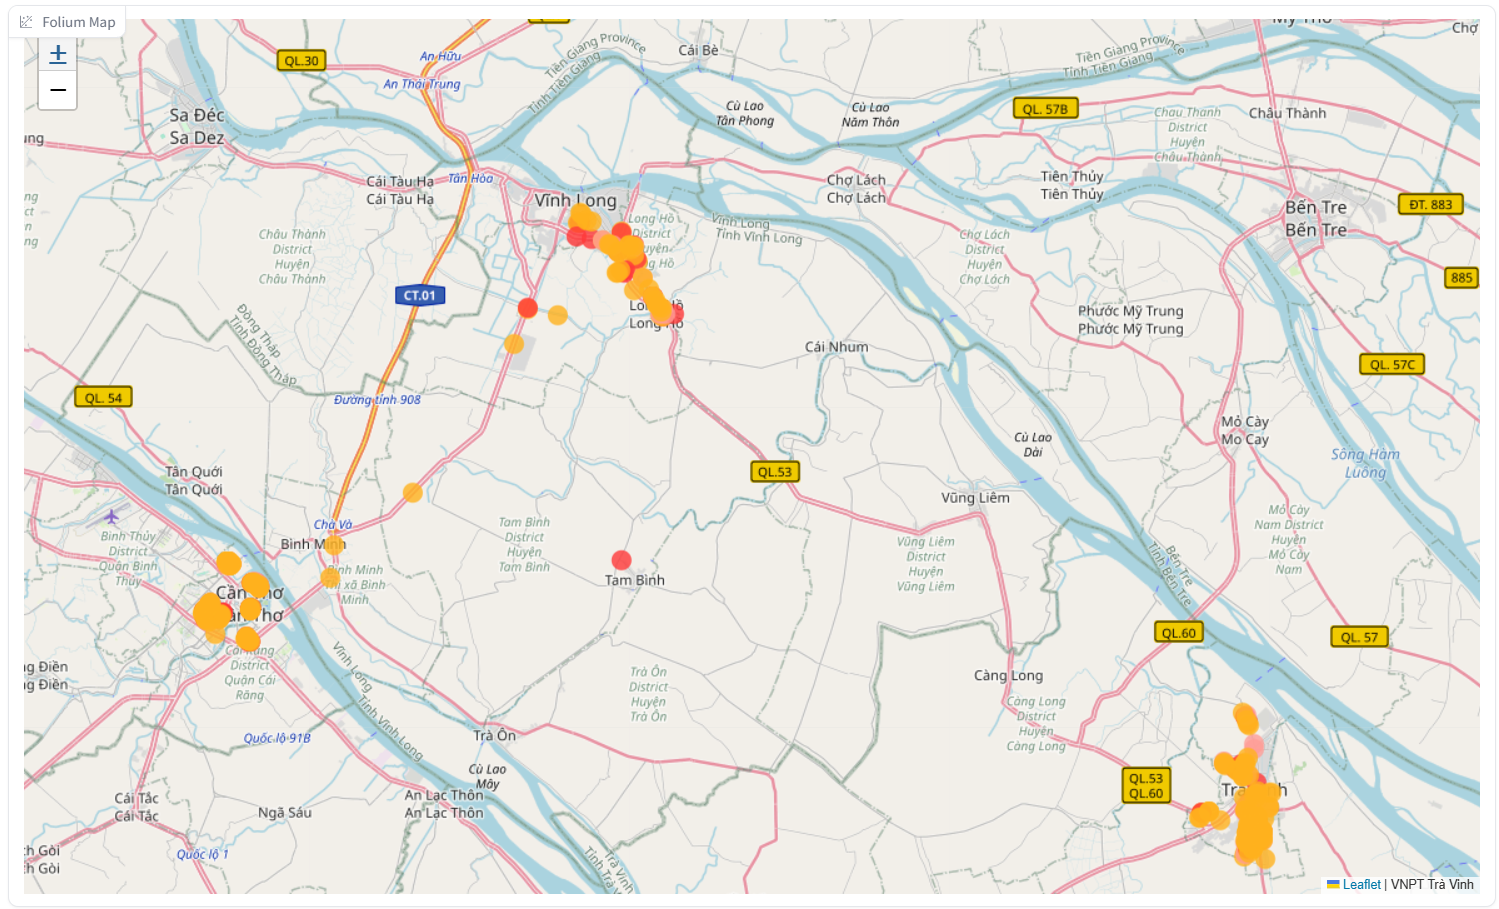
\includegraphics[width=1\textwidth]{demo2.png}
    \caption{Bản đồ phân bố các địa điểm có rác được phân loại ở ba tỉnh Vĩnh Long, Cần Thơ, Trà Vinh}
    \label{fig:demo2}
\end{figure}


\begin{figure}[H]
    \centering
    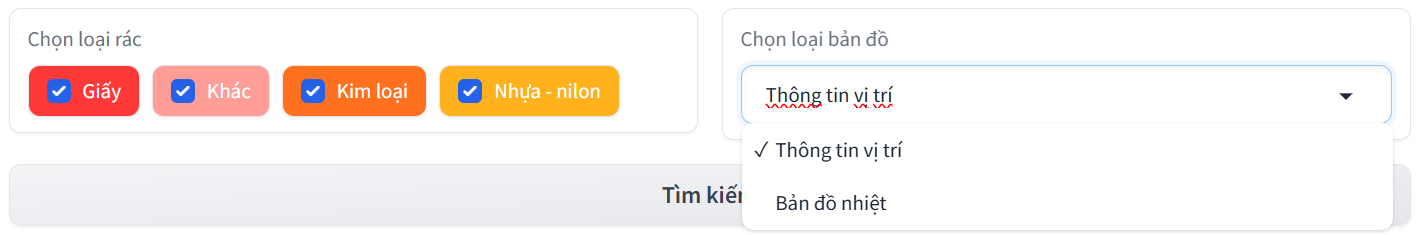
\includegraphics[width=1\textwidth]{demo2.1.png}
    \caption{Hình ảnh về các tùy chọn loại rác và loại bản đồ của hệ thống}
    \label{fig:demo2.1}
\end{figure}

{\fontsize{13}{12} \selectfont 

Đối với loại bản đồ thông tin vị trí, các chấm tròn là đại diện của lớp rác có số lượng cao nhất được phát hiện. Mỗi chấm tròn cung cấp thông tin địa lý, hình ảnh, số lượng rác của mỗi loại mà hệ thống phát hiện được và ngày chụp hình ảnh, 
như Hình \ref{fig:demo3} thể hiện thông tin số lượng với lớp nhựa - nilon là 1, giấy là 2, kim loại là 1 và 1 loại khác, ngoài ra còn có thông tin cụ thể về địa chỉ chụp ảnh và ngày chụp giúp xác định được vị trí và thời gian của hình.
Đối với loại bản đồ nhiệt, bản đồ thể hiện mức độ tổng quan về mức độ phân bố tập trung của các loại rác, người dùng sẽ theo dõi được khu vực hiện đang tập trung nhiều rác mà hệ thống cung cấp (xem Hình \ref{fig:demo4}).

}

\begin{figure}[H]
    \centering
    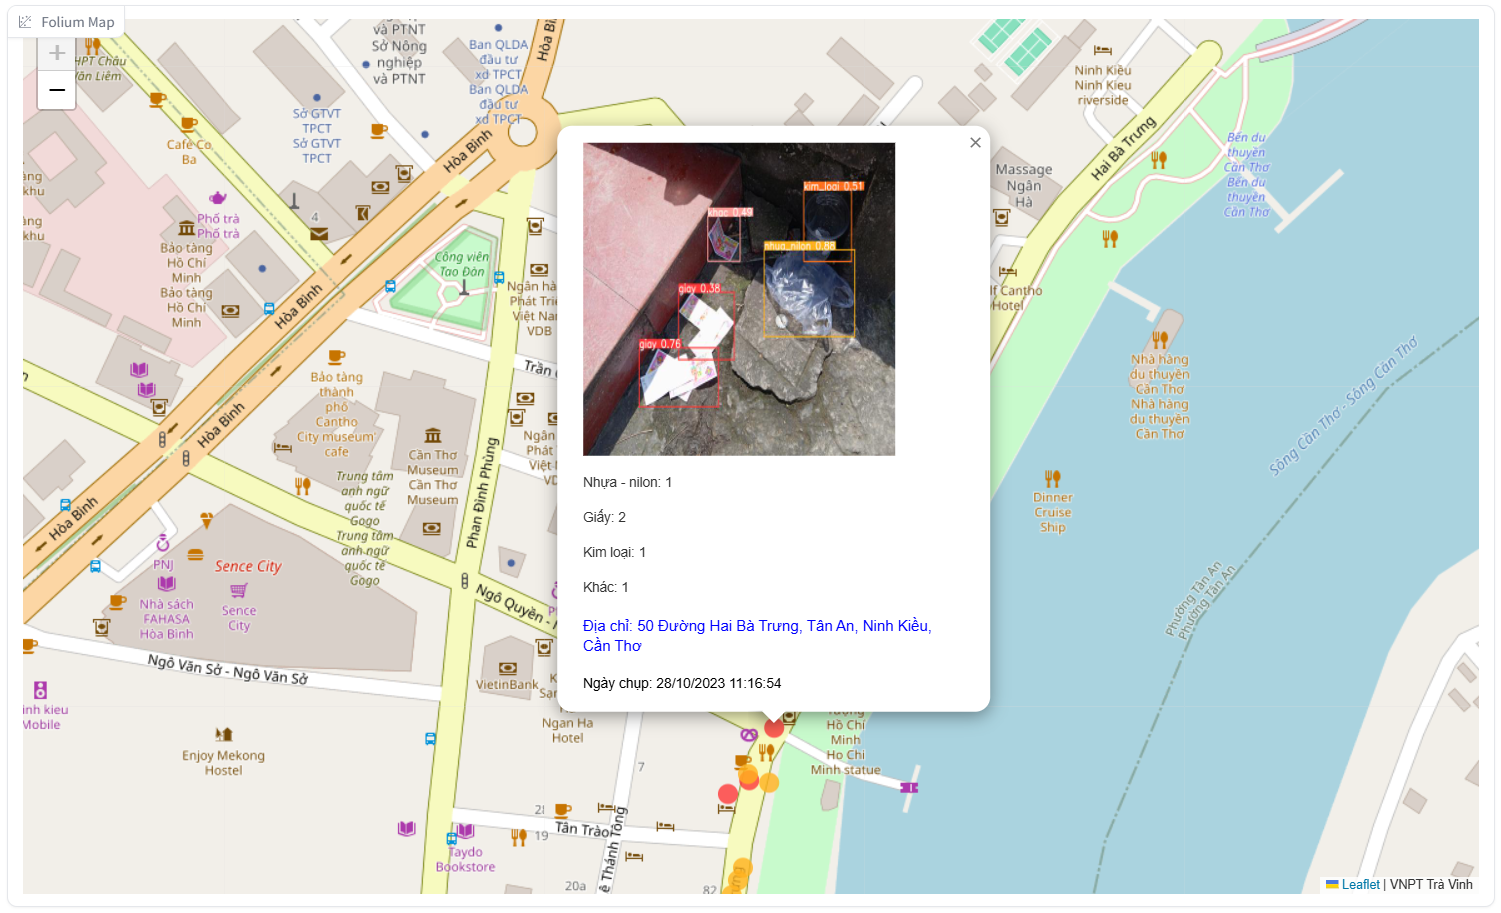
\includegraphics[width=1\textwidth]{demo3.png}
    \caption{Hình ảnh chi tiết mỗi điểm của bản đồ phân bố}
    \label{fig:demo3}
\end{figure}


\begin{figure}[H]
    \centering
    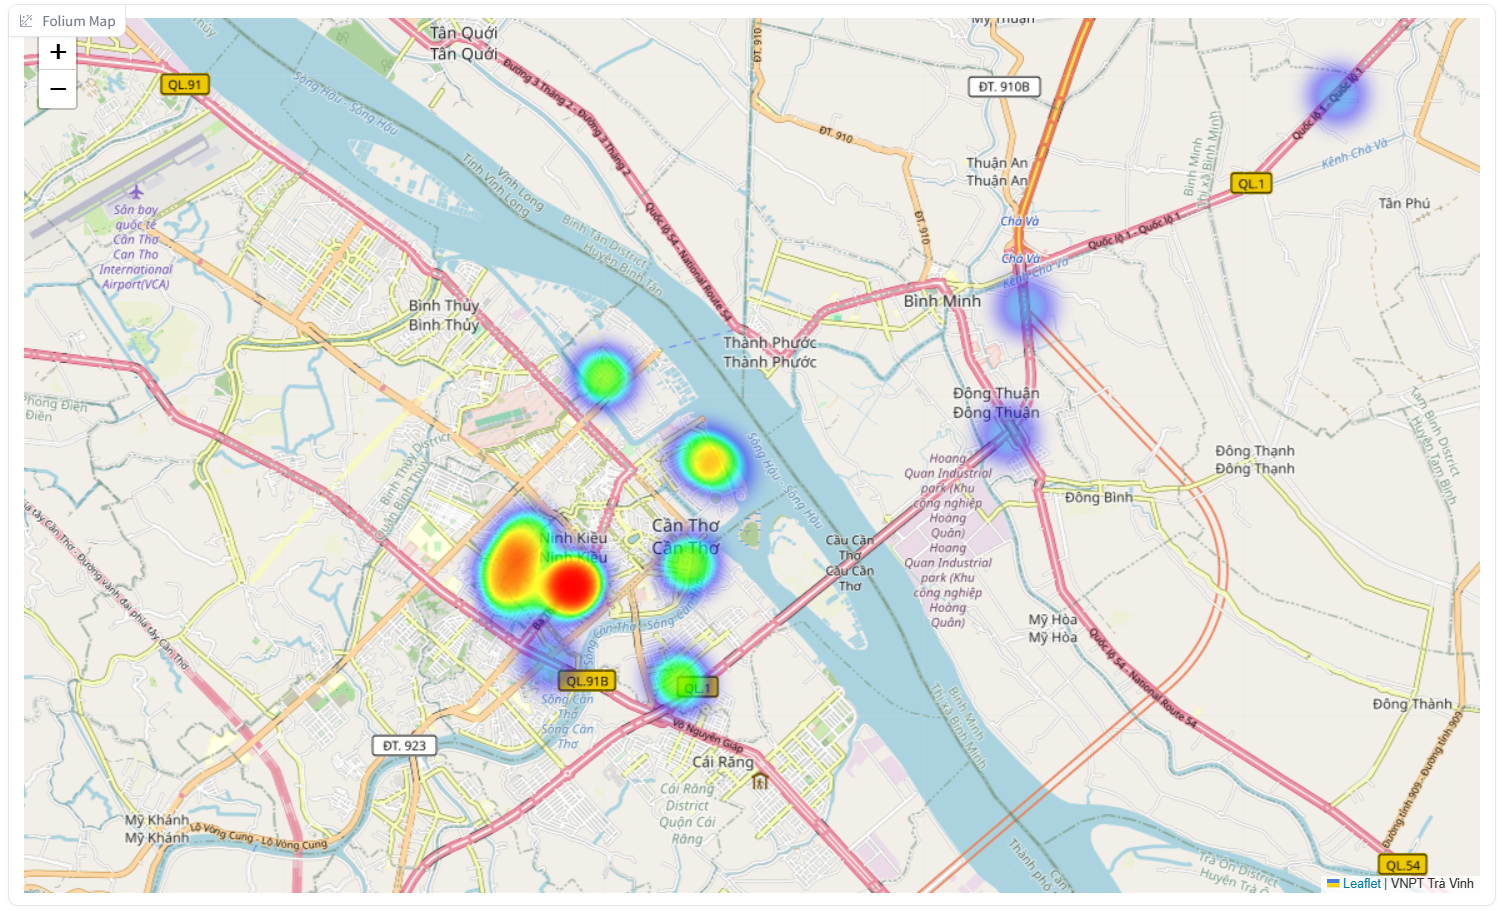
\includegraphics[width=1\textwidth]{demo4.png}
    \caption{Hình ảnh bản đồ nhiệt về các khu vực phân bố rác}
    \label{fig:demo4}
\end{figure}

{\fontsize{13}{12} \selectfont 
Thông tin trên bản đồ giúp các nhà quản lý có kế hoạch thu gom rác phù hợp, tránh tình trạng rác bị tích tụ. 
Ngoài ra, hệ thống là tiền đề phát triển thêm các chức năng như kết nối tới trung tâm giám sát để theo dõi hiệu suất và phản hồi từ người dùng bằng việc triển khai trên ứng dụng di động.
Các dữ liệu thu thập từ người dùng sử dụng hệ thống có thể sử dụng cho mục đích tối ưu hóa mô hình, giúp tăng hiệu suất phát hiện. 

}


\end{document}